\begin{document}
\begin{titlepage}

\begin{center}

{\small\textsc{Нижегородский государственный университет имени Н.\,И. Лобачевского}}
\vskip 1pt \hrule \vskip 3pt
{\small\textsc{Радиофизический факультет}}

\vfill

{\Large Отчет по лабораторной работе №\labnumber\vskip 12pt\bfseries \labtheme}
	
\end{center}

\vfill
	
\begin{flushright}
	{Выполнили студенты \labgroup\ группы\\ \labauthors}%\vskip 12pt Принял:\\ Менсов С.\,Н.}
\end{flushright}
	
\vfill
	
\begin{center}
	Нижний Новгород, \the\year
\end{center}

\end{titlepage}


\newpage
%!TEX root = ../HarmonicGenerator.tex
\thispagestyle{empty}
УДК 621.391


Генератор гармонических колебаний: для студентов-радиофизиков/ 
\noindent

Сост.А.В.Силин, Е.И.Шкелев.
-Н.Новгород: ННГУ, 1994.-25с

\vfill
Методические указания содержат: краткое изложение принципа работы схемы автогенератора; описание экспериментальной установки и задание к выполнению работы.

Адресовано студентам-радиофизикам.
\vfill

\begin{center}
	Составители: 

	канд.тех.наук А.В.Силин
	
	канд.тех.наук Е.И.Шкелев
\end{center}
\vfill
\begin{flushleft}
Нижегородский государственный университет \\
им. Н.И. Лобачевского, 1994
\end{flushleft}
\newpage
%\tableofcontents
\section{Цель работы}
Ознакомление с устройством генератора гармонических колебаний.

\section{Назначение автогенератора}
Данное устройство служит источником незатухающих колебаний синусоидальной формы с управляемой частотой.

\section{Области использования}
Автогенераторы находят широкое применение в радиотехнике (возбудители в радиопередатчиках, гетеродины в радиоприемниках), в измерительной технике (задающие генераторы в генераторах стандартных сигналов, опорные генераторы в схемах автоподстройки частоты), в устройствах автоматики и электронной техники (например, в электронных часах) и т.д.
К наиболее важным техническим характеристикам автогенераторов относятся: диапазон рабочих частот, стабильность и точность выставления частоты, уровень гармоник в спектре выходного сигнала, уровень выходного сигнала.

\section{Принцип работы схемы автогенератора}
Любой автогенератор представляет собой нелинейное устройство, преобразующее энергию источника питания (источника постоянного напряжения) в энергию колебаний. При широком разнообразии известных схем автогенераторов каждая из них, помимо источника питания, должна иметь усилитель и цепь обратной связи. Поэтому в обобщенном виде схема автогенератора (см. рис.\ref{fig:fig1}) содержит четырехполюсник в прямой цепи, соответствующий резонансному усилителю, и четырехполюсник в обратной цепи. (Обратите внимание на взаимное расположение входов и выходов четырехполюсников).
\begin{figure}[h]
	\centering
	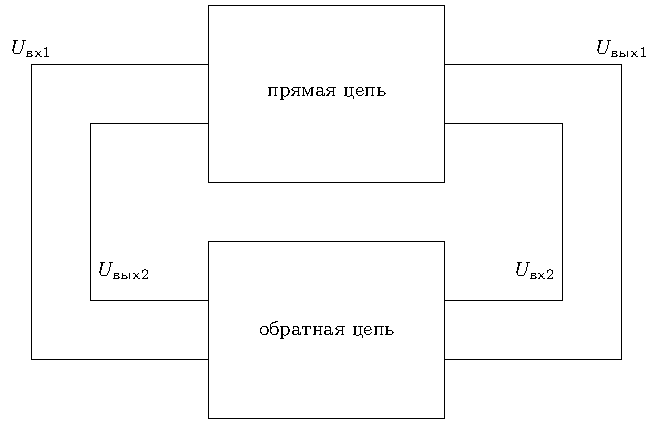
\includegraphics[width=0.5\linewidth]{circuit/one.pdf}
	\caption{}
	\label{fig:fig1}
\end{figure}
Простейшая схема автогенератора (схема с трансформаторной обратной связью), где в качестве активного элемента резонансного усилителя использован транзистор, приведена на рис.\ref{fig:fig2}. На рис.\ref{fig:fig2} пунктиром выделен четырехполюсник обратной связи.

При изучении автогенератора первостепенное значение имеют два вопроса:
\begin{enumerate}
\item Механизм и условия возникновения колебаний.
\item Существование стационарных колебаний и их устойчивость
\end{enumerate}

\begin{figure}[h]
	\centering
	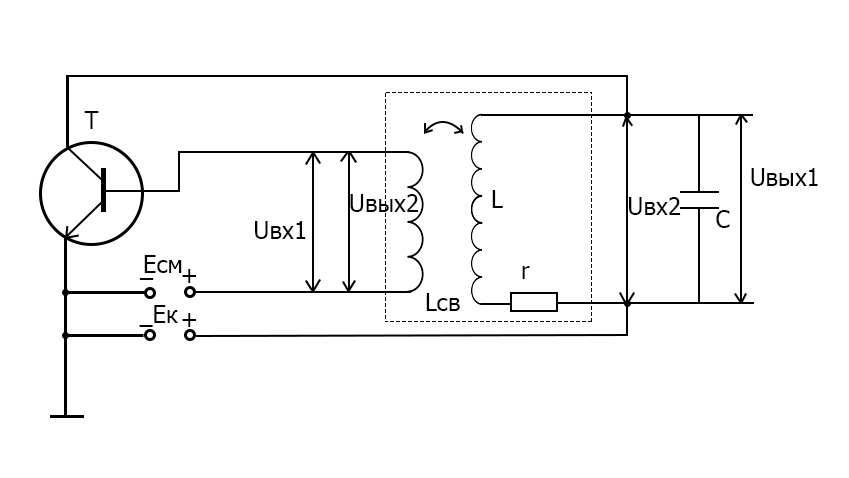
\includegraphics[width=0.8\linewidth]{circuit/fig2}
	\caption{}
	\label{fig:fig2}
\end{figure}

\section{Самовозбуждение автогенератора}
При включении в схему автогенератора (рис.\ref{fig:fig2}) источников питания и при выполнении далее обсуждаемых условий в схеме возникают автоколебания. Механизм их возникновения заключается в следующем. Скачок напряжения на коллекторе приведет к быстрому изменению выходного тока транзистора, что вызовет ударное возбуждение резонансного контура. Возникшие в контуре колебания через трансформаторную связь проникают на базу транзистора и вызовут переменную составляющую выходного тока. При соответствующих условиях этот ток будет в фазе с током в резонансном контуре, и в результате возникшие за счет скачка напряжения питания собственные колебания в контуре могут со временем не только не ослабевать, но и усиливаться. По мере увеличения уровня колебаний все в большей степени будет проявляться нелинейность характеристик транзистора, что, в свою очередь, приведет к снижению скорости нарастания колебаний в контуре, а затем и к прекращению их роста - колебания приобретают стационарный характер.

При возникновении автоколебаний их уровень на некотором начальном интервале времени остается весьма малым. По этой причине при обсуждении условий самовозбуждения можно пользоваться линейной моделью в виде двух линейных четырехполюсников, соединенных по схеме на рис.\ref{fig:fig1}. Обозначим через $\dot{K}_{1(\omega)}$ и $\dot{K}_{2(\omega)}$ комплексные коэффициенты передачи четырехполюсников прямой и обратной цепи соответственно
\begin{equation*}
\begin{aligned}
&\dot{K}_1(\omega)=\frac{\dot{U}_{\text{вых}1}}{\dot{U}_{\text{вх}1}} \\
&\dot{K}_2(\omega)=\frac{\dot{U}_{\text{вых}2}}{\dot{U}_{\text{вх}2}} 
\end{aligned}
\end{equation*}
где $\dot{U}$ - комплексная амплитуда.

\begin{figure}[h]
	\centering
	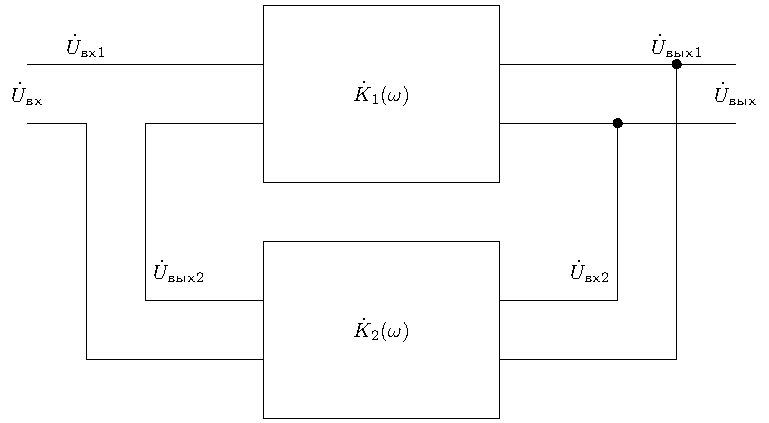
\includegraphics[width=0.6\linewidth]{circuit/two.pdf}
	\caption{}
	\label{fig:fig3}
\end{figure}

Перерисуем схему рис.\ref{fig:fig1} в более удобном для обсуждения виде (см.рис.\ref{fig:fig3}). Легко заметить, что при $\dot{U}_\text{вх}=0$, схемы на рис.\ref{fig:fig1} и рис.\ref{fig:fig3} совпадают.

Для линейного четырехполюсника (рис.\ref{fig:fig3}) введем комплексный коэффициент передачи $\dot{K}(\omega)$
\begin{equation*}
\dot{K}(\omega)=\frac{\dot{U}_\text{вых}}{\dot{U}_\text{вх}}.
\end{equation*}
Поскольку
\begin{equation*}
\begin{aligned}
&\dot{U}_\text{вых}=\dot{U}_{\text{вых}1}=\dot{U}_{\text{вх}1}\dot{K}_1(\omega)=\\
&= [\dot{U}_{\text{вх}1}+\dot{K}_2(\omega)\dot{U}_{\text{вых}1}]\dot{K}_1(\omega),
\end{aligned}
\end{equation*}
то 
\begin{equation*}
\dot{K}(\omega)=\frac{\dot{K}_1(\omega)}{1-\dot{K}_1(\omega)\dot{K}_2(\omega)}.
\end{equation*}

Наличие особой точки у комплексной функции $\dot{K}(\omega)$ при условии $1-\dot{K}_1(\omega)\dot{K}_2(\omega)$ физически можно интерпретировать следующим образом: схема на рис.\ref{fig:fig3} при выполнении условия $1-\dot{K}_1(\omega)\dot{K}_2(\omega)$ выдает на выходе колебание с ненулевой амплитудой при бесконечно малой (нулевой) амплитуде колебания на входе. Следовательно, схема  на рис.\ref{fig:fig3} при названных условиях является автогенератором.

Условия самовозбуждения вытекают из равенства
\begin{equation*}
1-\dot{K}_1(\omega)\dot{K}_2(\omega)=0.
\end{equation*}

Отсюда 
\begin{equation}
\begin{aligned}
& |\dot{K}_1(\omega)||\dot{K}_2(\omega)|=1, & \phi_1(\omega)+\phi_2(\omega)=2\pi n,
\end{aligned}
\label{eq:1}
\end{equation}
где $\phi_1(\omega)$ и $\phi_2(\omega)$ - аргументы функций $\dot{K}_1(\omega)$ и $\dot{K}_2(\omega)$; $n$ - целое число. Первое условие получило название "баланс амплитуд", второе - "баланс фаз".

Равенства (\ref{eq:1}) можно рассматривать как уравнения относительно переменной $\omega$. Корни этих уравнений являются теми частотами, на которых возможно возбуждение. Частота генерации - корень системы уравнений \eqref{eq:1}.

Таким образом, если в схеме автогенератора на какой-либо частоте $\omega^*$ модуль комплексного коэффициента передачи разомкнутого кольца обратной связи $|\dot{K}_1(\omega)||\dot{K}_2(\omega)|$ равен 1, а суммарный набег фаз при прохождении сигнала с этой частотой по тому же кольцу составит $2\pi n$, то в схеме произойдет самовозбуждение. Частота генерируемых колебаний будет равна $\omega^*$.

Выполнение условий самовозбуждения, по существу, означает, что возникшие колебания схемой автогенератора будут поддерживаться на неизменном уровне; неизбежные потери в кольце обратной связи полностью скомпенсированы.

Если условие $|\dot{K}_1(\omega)||\dot{K}_2(\omega)|=1$ не выполнено, имеем
\begin{enumerate}
\item {
	$|\dot{K}_1(\omega)||\dot{K}_2(\omega)|=0$ при $\dot{K}_2(\omega)=0$ - резонансный усилитель;
}
\item {
	$|\dot{K}_1(\omega)||\dot{K}_2(\omega)|<1$ при $\phi_1(\omega)+\phi_2(\omega)=2\pi n$ - регенеративный усилитель;
}
\item {
	$|\dot{K}_1(\omega)||\dot{K}_2(\omega)|>1$ при $\phi_1(\omega)+\phi_2(\omega)=2\pi n$ - генератор нарастающих колебаний.
}
\end{enumerate}
Рассмотрим каждый из этих случаев.

\subsection{Резонансный усилитель}
При малом уровне входного сигнала усилитель работает в линейном режиме: $\dot{K}(\omega)$ является его исчерпывающей характеристикой.
При возрастании амплитуды входного колебания $U_\text{вх}(t)=U_0\cos \omega_0 t$ линейность усилителя будет нарушена. Аппроксимируя проходную динамическую характеристику транзистора $i_k=f(U_\text{вх})$ степенным полиномом степени $N$, выходной ток усилительного каскада можно записать в виде
\begin{equation}
i_\text{вых}=\sum\limits_{n=0}^{N}b_n U^n_\text{вх},
\label{eq:2}
\end{equation}
где $b_n$ - постоянные коэффициенты.
Подставив в \eqref{eq:2} выражение для $U_\text{вх}(t)$, находим амплитуду первой гармоники выходного тока в виде
\begin{equation}
I_1=U_0[b_1+\frac{3}{4}b_3U_0^2+\frac{5}{8}b_5U_0^4+\ldots],
\label{eq:3}
\end{equation}

По аналогии с линейным случаем, где $I_1=S_0U_0$, $S_0$ - крутизна в рабочей точке, для нелинейного усилителя можно записать 
\begin{equation}
I_1=S_\text{ср}(U_0)\cdot U_0
\label{eq:4}
\end{equation}
$S_\text{ср}(U_0)$ - средняя крутизна, которая находится из \eqref{eq:3} в соответствии с определением $S_\text{ср}(U_0)=I_1/U_0$:
\begin{equation}
S_\text{ср}(U_0)=b_1+\frac{3}{4}b_3U_0^2+\frac{5}{8}b_5U_0^4+\ldots.
\label{eq:5}
\end{equation}

Как следует из \eqref{eq:5}, зависимость $S_\text{ср}(U_0)$ полностью определяется коэффициентом аппроксимирующего полинома $b_{2n+1}$, а сами коэффициенты зависят как от типа электронного прибора и нагрузки, так и от режима его работы.

Чтобы выяснить характер зависимость $S_\text{ср}(U_0)$, рассмотрим рис.\ref{fig:fig4}a, где изображены проходная характеристика транзистора и ее крутизна.

\begin{center}
    \begin{figure}[H]
        \vspace{-10pt}
        \begin{minipage}{0.49\linewidth}
            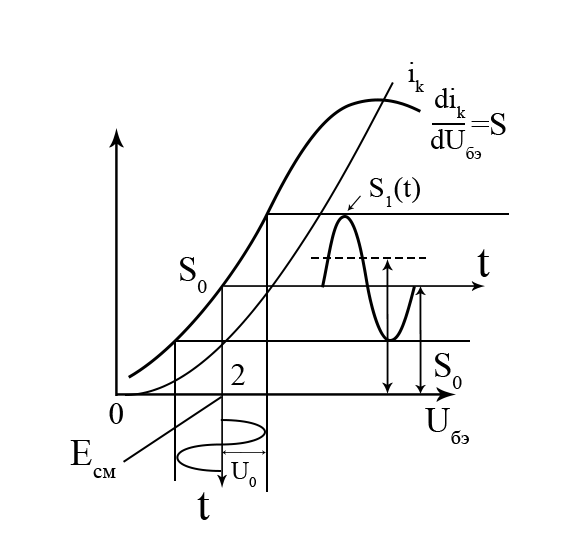
\includegraphics[width=\linewidth]{circuit/fig4a} 
            \vspace{-50pt}
            \label{fig:4a}
            \captionof{subfigure}{} 
        \end{minipage}
    \begin{minipage}{0.49\linewidth}
        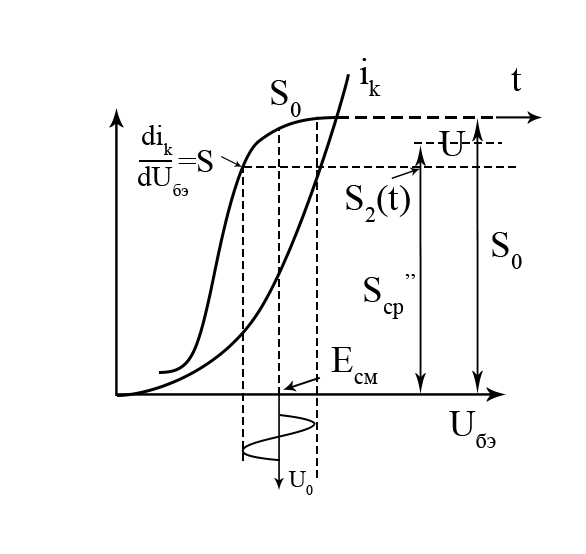
\includegraphics[width=\linewidth]{circuit/fig4b} 
        \vspace{-50pt}
        \label{fig:4b}
        \captionof{subfigure}{} 
    \end{minipage}
    \caption{}
    \vspace{-40pt}
    \label{fig:4}
    \end{figure}
\end{center} 

Различие рисунков \ref{fig:fig4}a и \ref{fig:fig4}б состоит в том, что в первом случае с помощью смещения $E_\text{см}$ рабочая точка выбрана на нелинейном участке проходной характеристики, во втором случае - на линейном, где в окрестности рабочей точки $S\approx\text{const}$. При воздействии на усилитель входного синусоидального напряжения с достаточно большой амплитудой $U_0$ крутизна характеристики описывается периодическими функциями времени $S_1(t)$ и $S_2(t)$, а постоянные составляющие $S'_\text{ср}$ и $S''_\text{ср}$ являются значениями средней крутизны, соответствующими амплитуде $U_0$. Нетрудно заметить, что при увеличении амплитуды входного колебания в случае рис.\ref{fig:fig4}а $S_\text{ср}(U_0)$ будет возрастать, в случае рис.\ref{fig:fig4}б - падать. На рис. \ref{fig:fig5} представлены два характерных вида зависимости $S_\text{ср}(U_0)$, при этом кривая 1 соответствует рис.\ref{fig:fig4}a, кривая 2 - рис.\ref{fig:fig4}б.

Зависимость \eqref{eq:4} амплитуды первой гармоники выходного тока $I_1$ от амплитуды колебания на входе $U_0$, получившая название "колебательной характеристики", в соответствии с кривыми на рис.\ref{fig:fig5} так же имеет два характерных вида. На рис.\ref{fig:fig6} - кривая 1 и 2 соответствуют кривым 1 и 2 на рис.\ref{fig:fig5}. Поскольку при настройке контура усилителя на частоту усиливаемого сигнала фаза напряжения на контуре совпадает с фазой первой гармоники тока, то кривые на рис.\ref{fig:fig6} отражают и характер зависимостей $U_k=f(U_0)$

\begin{figure}[h]
	\centering
	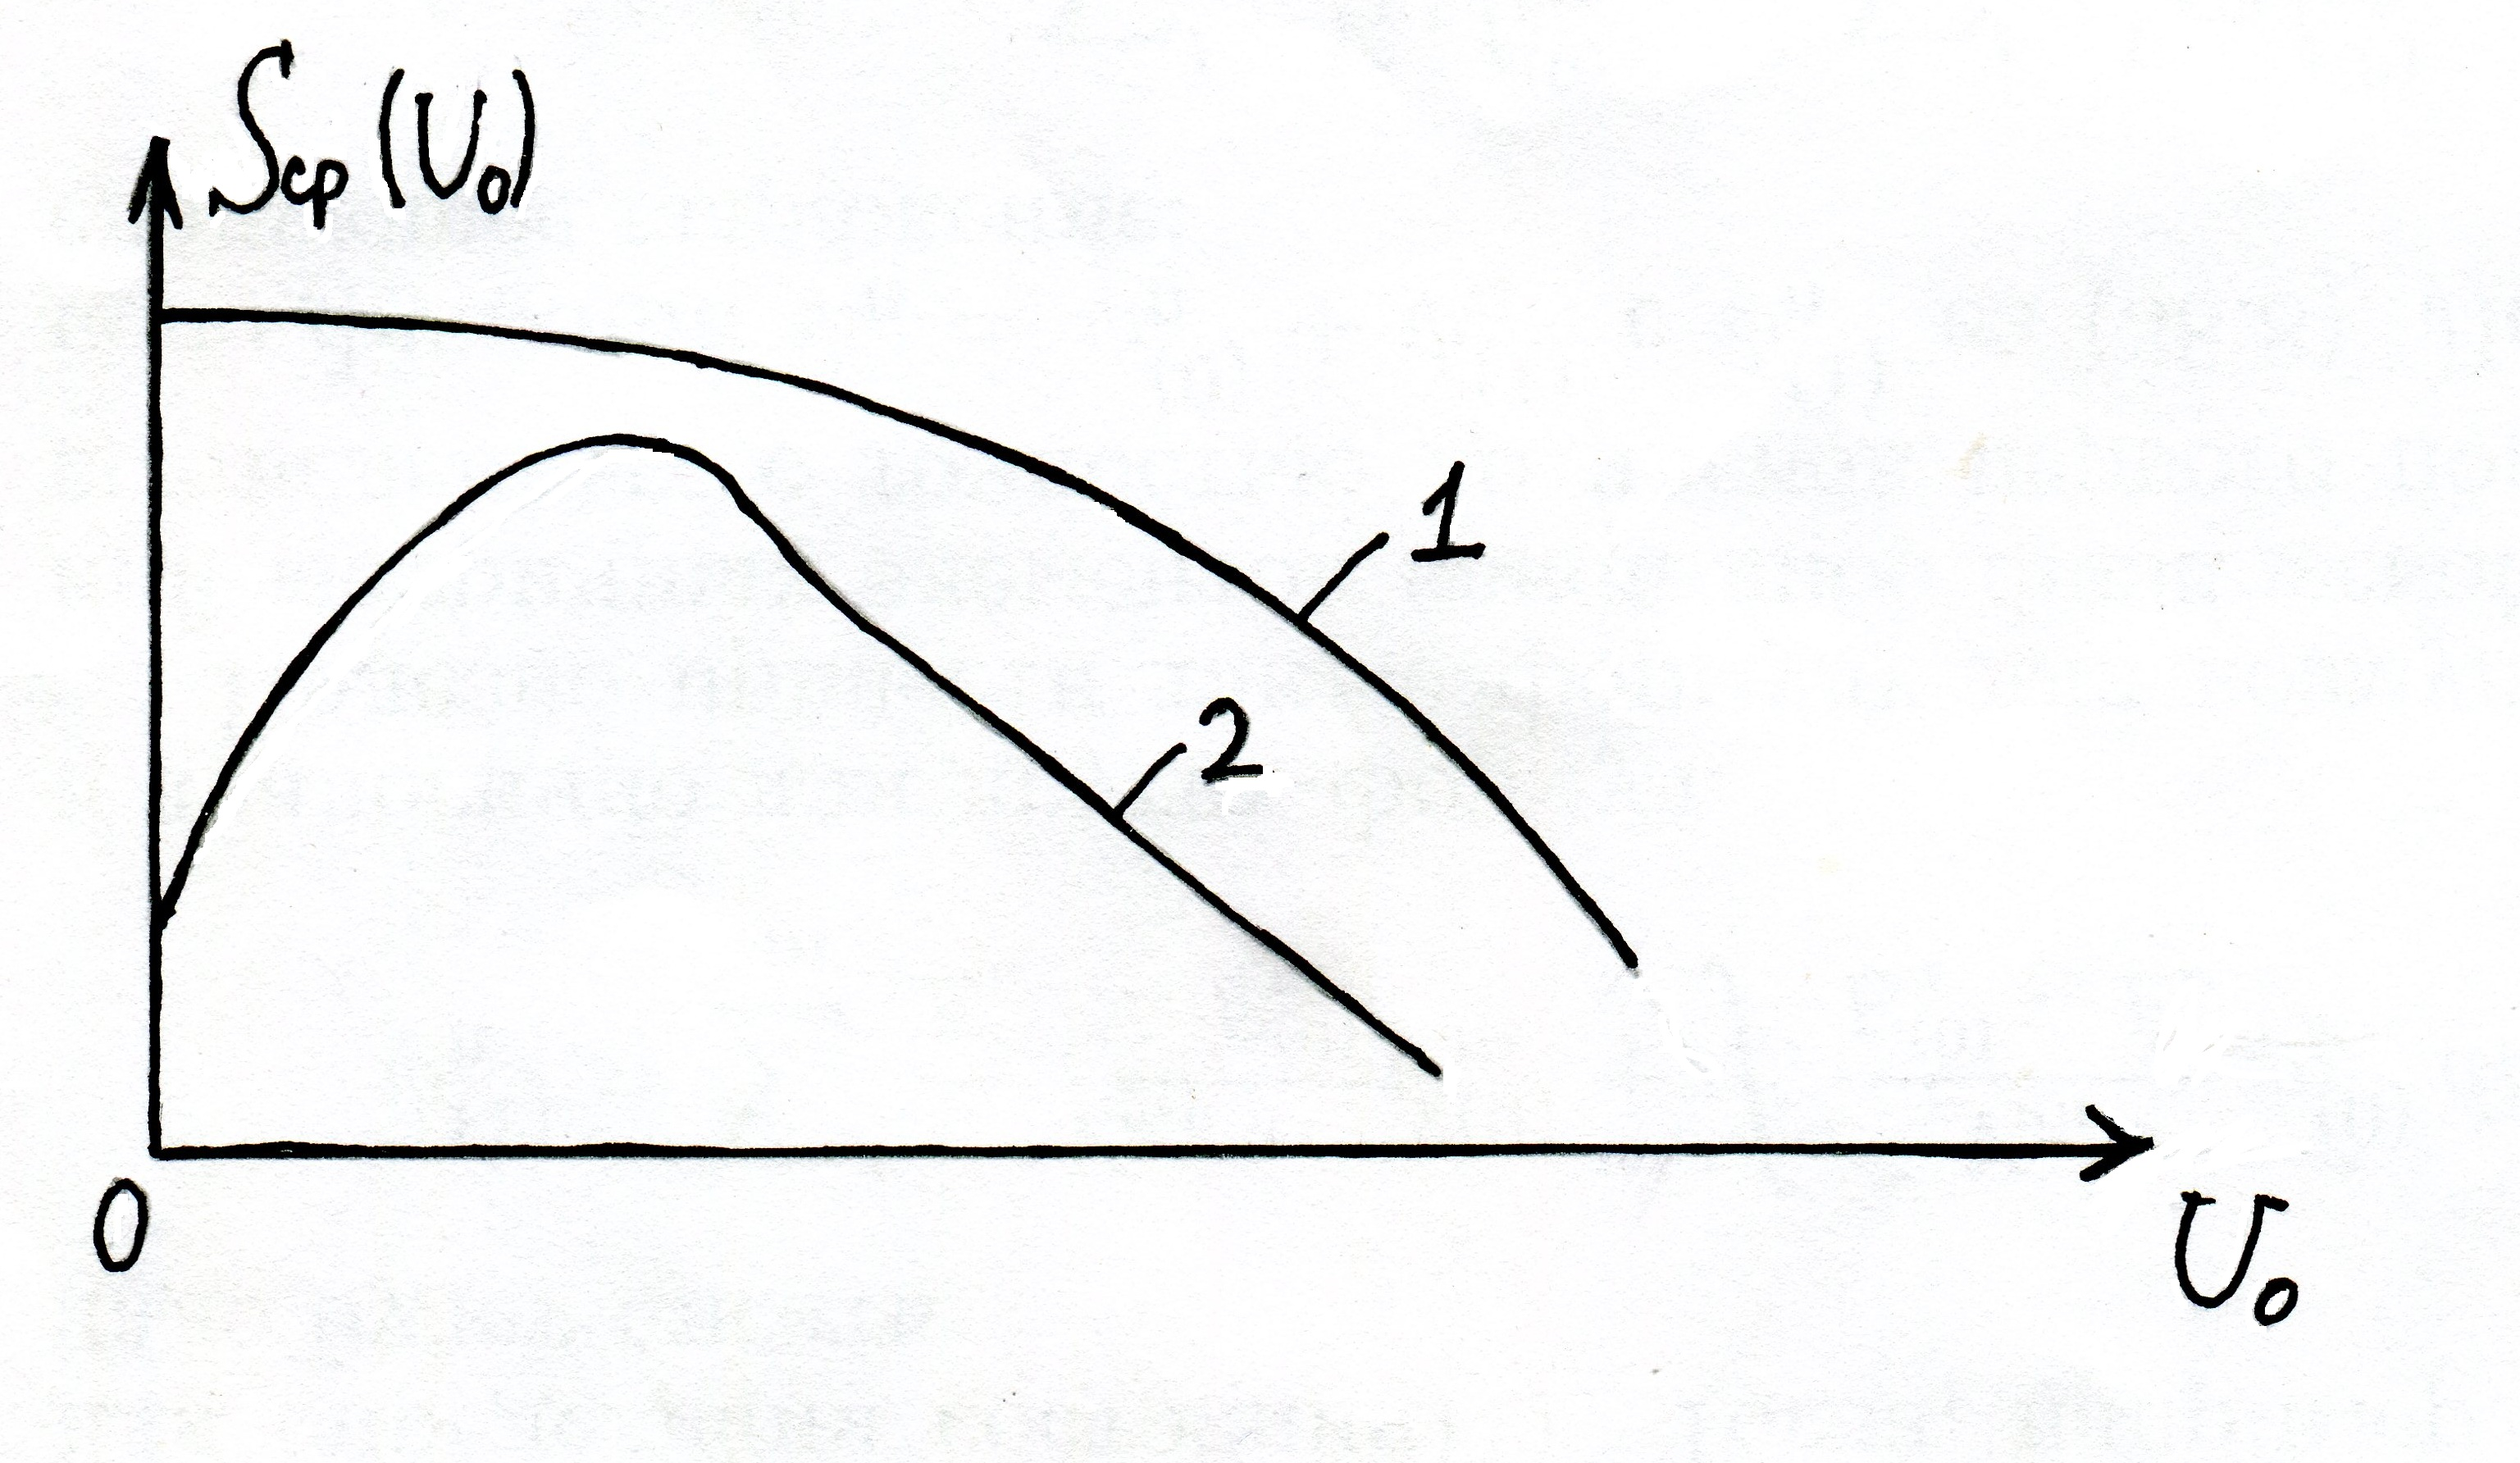
\includegraphics[width=0.4\linewidth]{circuit/fig5}
	\caption{}
	\label{fig:fig5}
\end{figure}

Коэффициент усиления по первой гармонике при работе усилителя в режиме большого сигнала $\dot{K}(\omega_0)$ в соответствии с \eqref{eq:4} и рис.\ref{fig:fig6} является зависимым от $U_0$.
\begin{equation}
\dot{K}(\omega)=\dot{U}_\text{вых}/\dot{U}_\text{вх}=U_k/U_\text{вх}=f(U_0).
\label{eq:6}
\end{equation}

\begin{figure}[h]
	\centering
	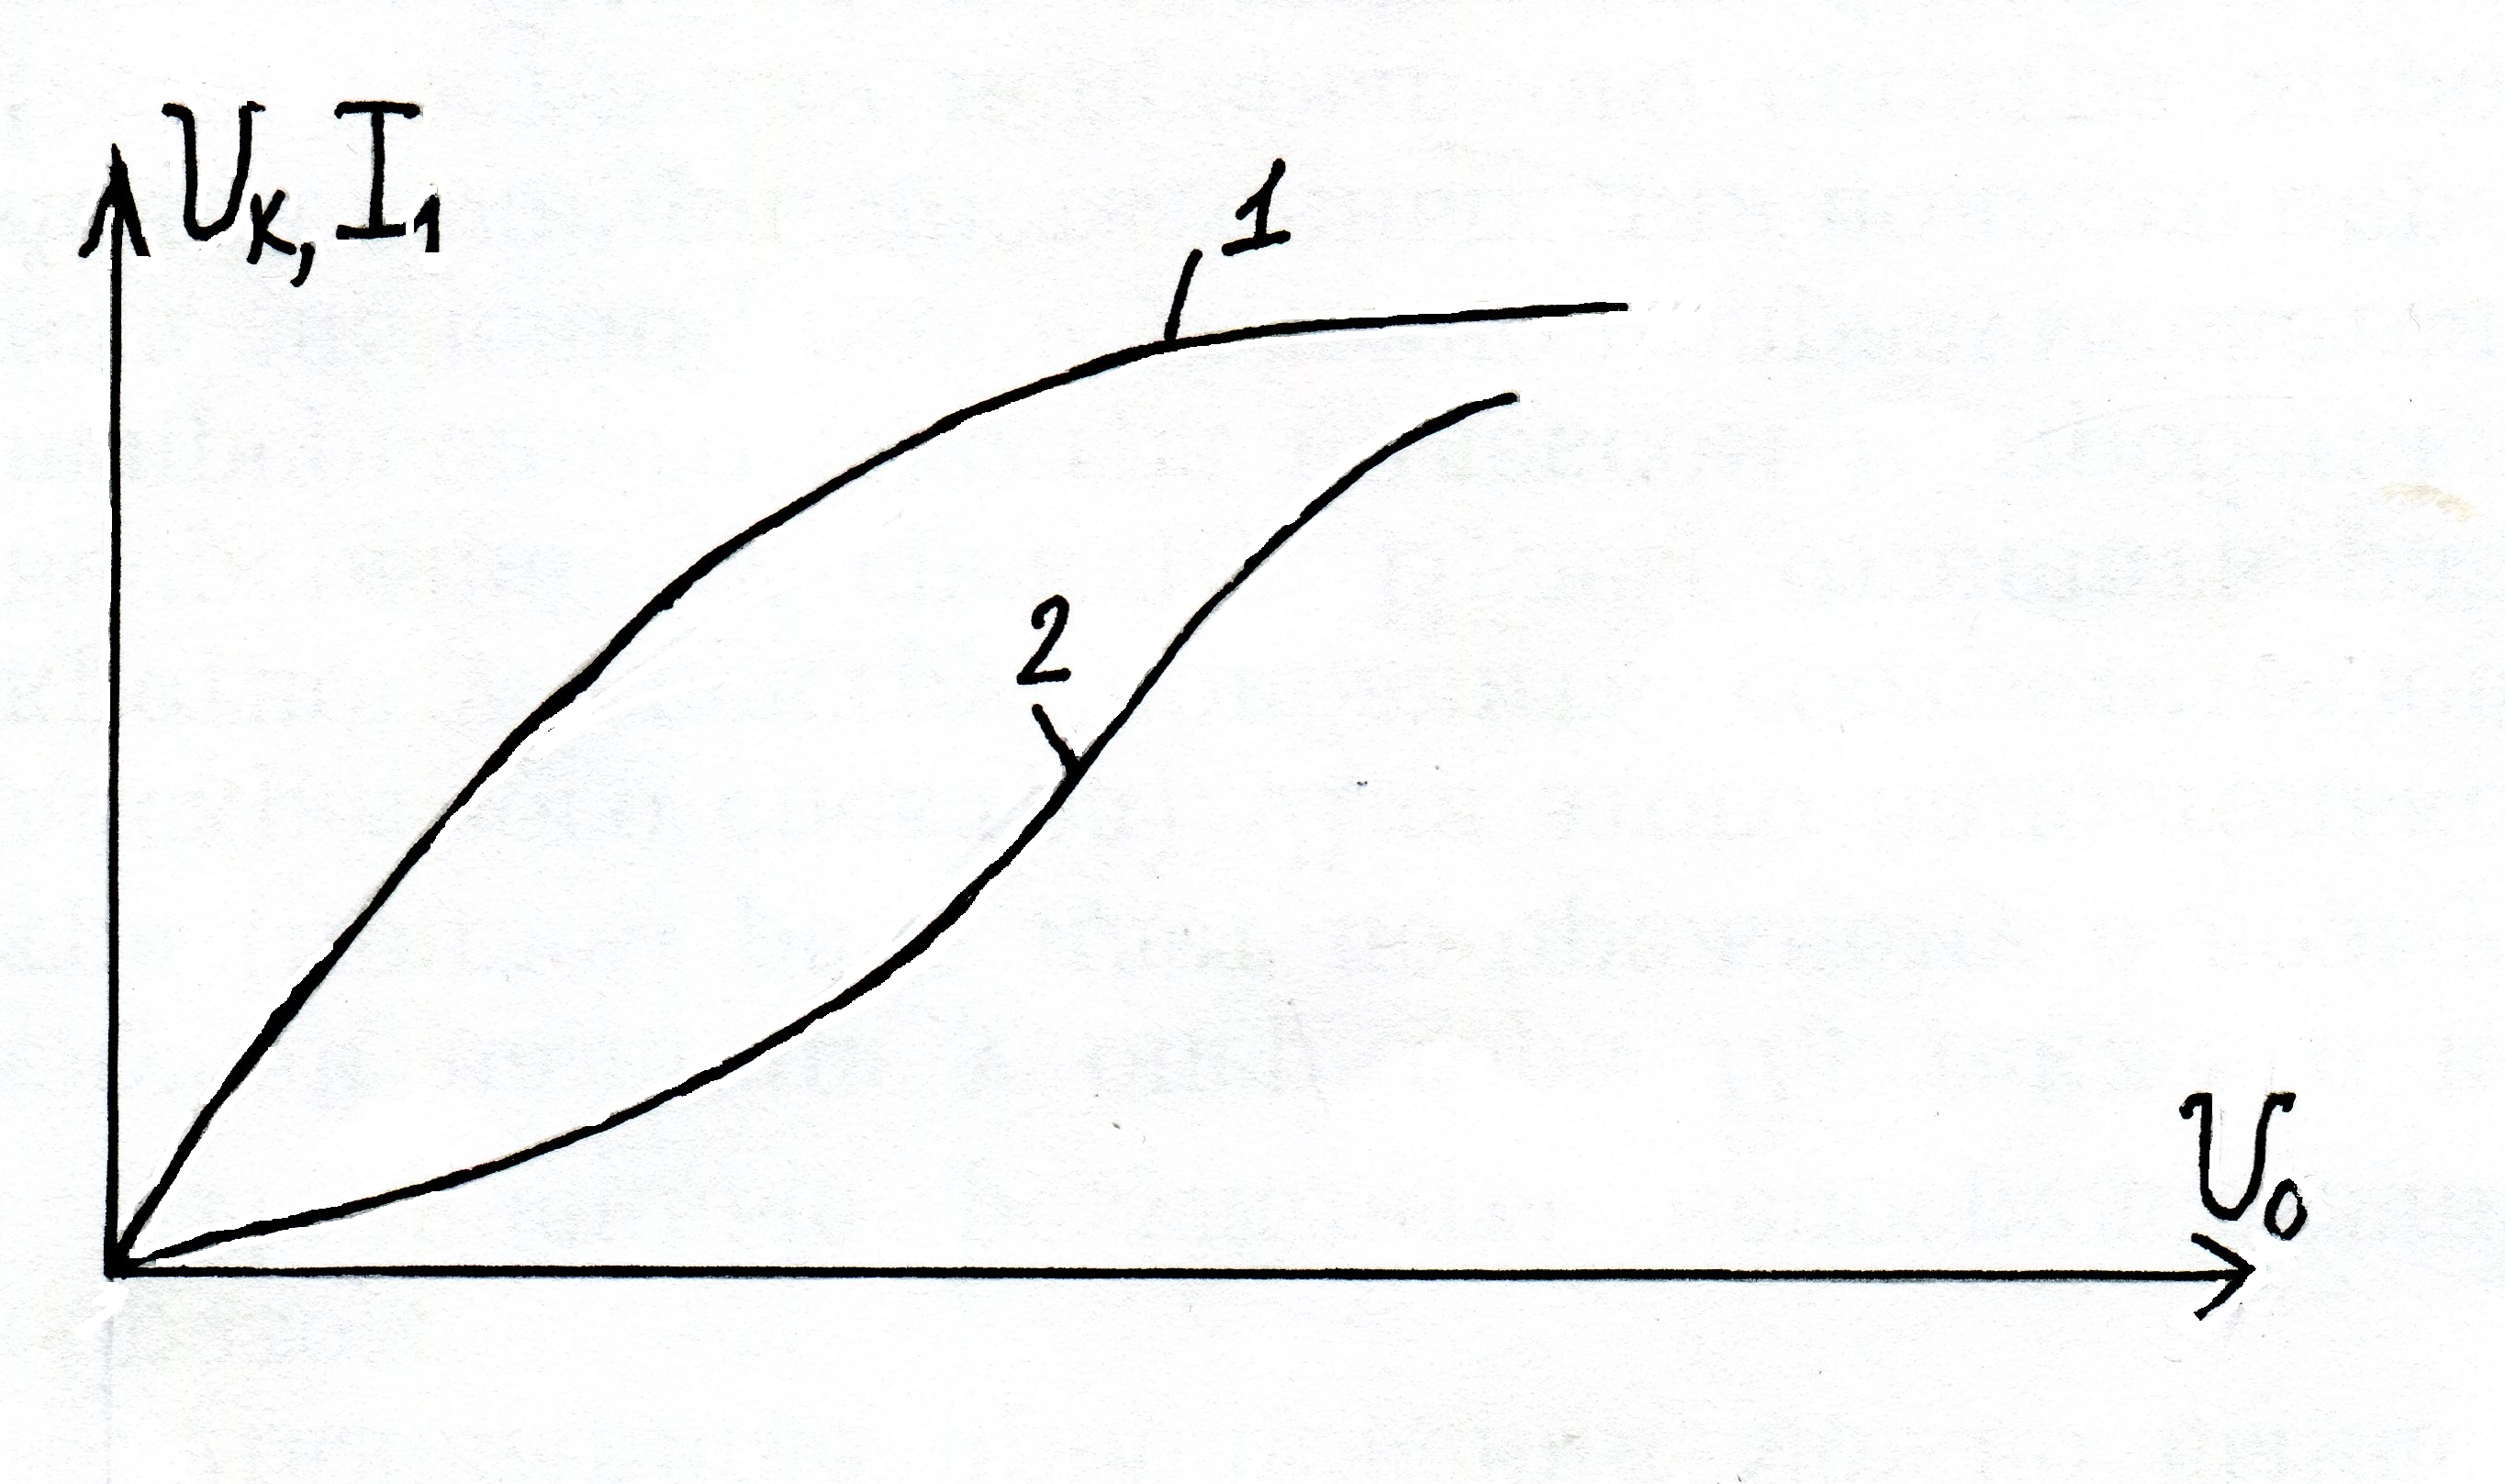
\includegraphics[width=0.4\linewidth]{circuit/fig6}
	\caption{}
	\label{fig:fig6}
\end{figure}

\subsection{Регенеративный усилитель}
При положительной обратной связи в усилителе, т.е. при $\phi_1(\omega)+\phi_2(\omega)=2\pi n$, при $0<|\dot{K}_1(\omega)||\dot{K}_2(\omega)|<1$ автоколебания в схеме на рис.\ref{fig:fig2} отсутствуют, а сама она представляет собой регенеративный усилитель. В радиотехнике под регенерацией подразумевается частичная компенсация потерь в колебательной системе с помощью положительной обратной связи. Явление регенерации позволяет повысить коэффициент усиления усилителя и его избирательность. Компенсация потерь увеличивает добротность контура. На рис.\ref{fig:figure7} иллюстрируется влияние степени связи(т.е. величины $|\dot{K}_2(\omega)|$) на усиления и избирательность.

\begin{figure}[h]
	\centering
	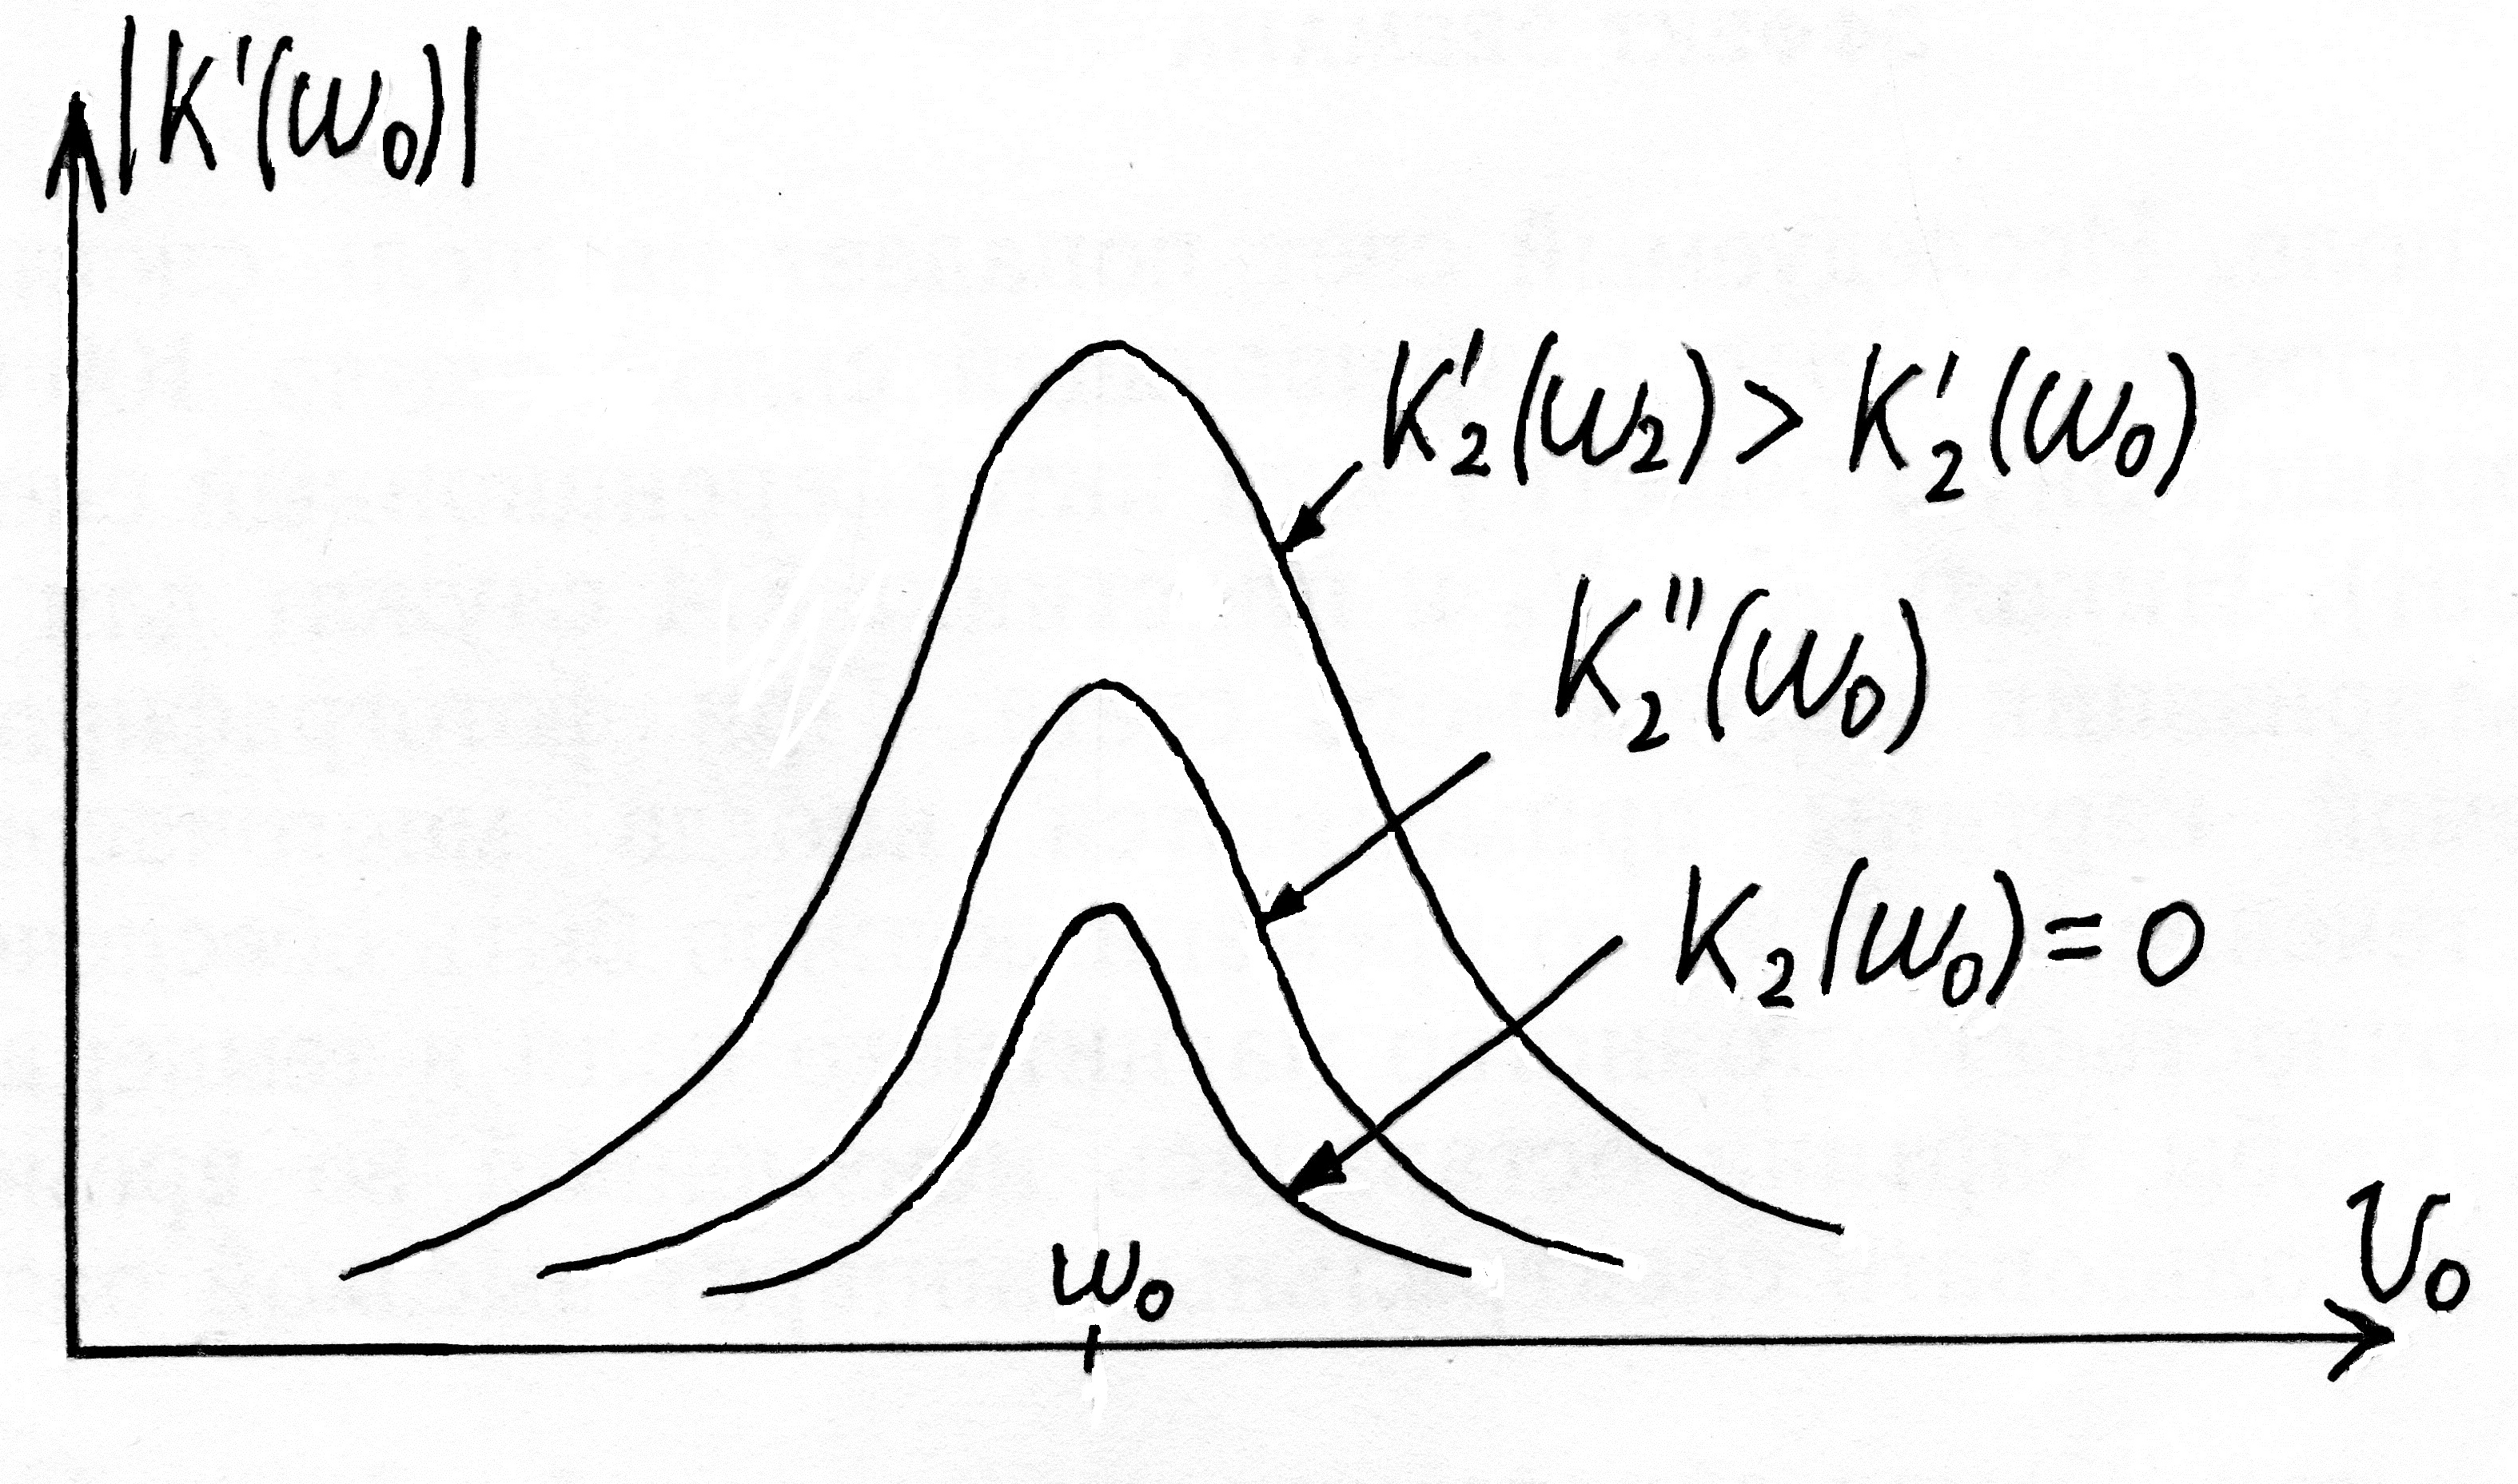
\includegraphics[width=0.4\linewidth]{circuit/fig7}
	\caption{}
	\label{fig:fig7}
\end{figure}

Наряду с отмеченными положительными свойствами регенеративного усилителя, ему свойственен и существенный недостаток - опасность возбуждения усилителя за счет случайных изменений $K_1(\omega)$.

\subsection{Ограничение нарастающих колебаний. Стационарный режим генератора} 
Строго говоря, выполнение условия $\dot{K}_1(\omega)\dot{K}_2(\omega)=1$, при $\phi_1(\omega)+\phi_2(\omega)=2\pi n$ означает лишь способность схемы на рис.\ref{fig:fig3} поддерживать незатухающие колебания, если они возникнут в ней за счет какого-либо внешнего воздействия. Для того, чтобы автоколебания достигли некоторого наперед заданного уровня необходимо обеспечить им нарастающий характер, что соответствует условию
\begin{equation*}
|\dot{K}_1(\omega)\dot{K}_2(\omega)|>1.
\end{equation*}

По мере роста амплитуды колебаний все в большей мере будет проявляться нелинейность усилителя в прямой цепи. При этом средняя крутизна в соответствии с рис.\ref{fig:fig5} будет уменьшаться, снижая $K_1(\omega_0)$. Снижение $K_1(\omega_0)$, в конечном итоге, приведет к тому, что будет выполнено условие
\begin{equation*}
\dot{K}_1(\omega_0)\dot{K}_2(\omega_0)=1.
\end{equation*}

На этом рост амплитуды колебаний прекратится: переходный режим завершится, наступит стационарный режим автогенератора.

Определение стационарной амплитуды колебаний удобно проводить с использованием колебательной характеристики (рис.\ref{fig:fig8})
На рис.\ref{fig:fig8} в одной системе координат представлены две зависимости (см.рис\ref{fig:fig2}) 
\begin{equation*}
U_{\text{вых}1}=K_1(\omega_0)U_{\text{вх}1}
\end{equation*}
- колебательная характеристика (кривая 1)
\begin{equation*}
U_{\text{вх}2}=\frac{1}{K_2(\omega_0)}U_{\text{вых}2}
\end{equation*}
или
\begin{equation*}
U_{\text{вых}1}=\frac{1}{K_2(\omega_0)}U_{\text{вх}1}
\end{equation*}
- прямая обратной связи (кривая 2).

Точка пересечения кривых 1 и 2 (точка $\alpha$) означает
\begin{equation*}
K_1(\omega_0)=\frac{1}{K_2(\omega_0)}
\end{equation*}
или
\begin{equation}
K_1(\omega_0)K_2(\omega_0)=1,
\label{eq:7}
\end{equation}
т.е. соответствует стационарной амплитуде автоколебаний.

\begin{figure}[h]
	\centering
	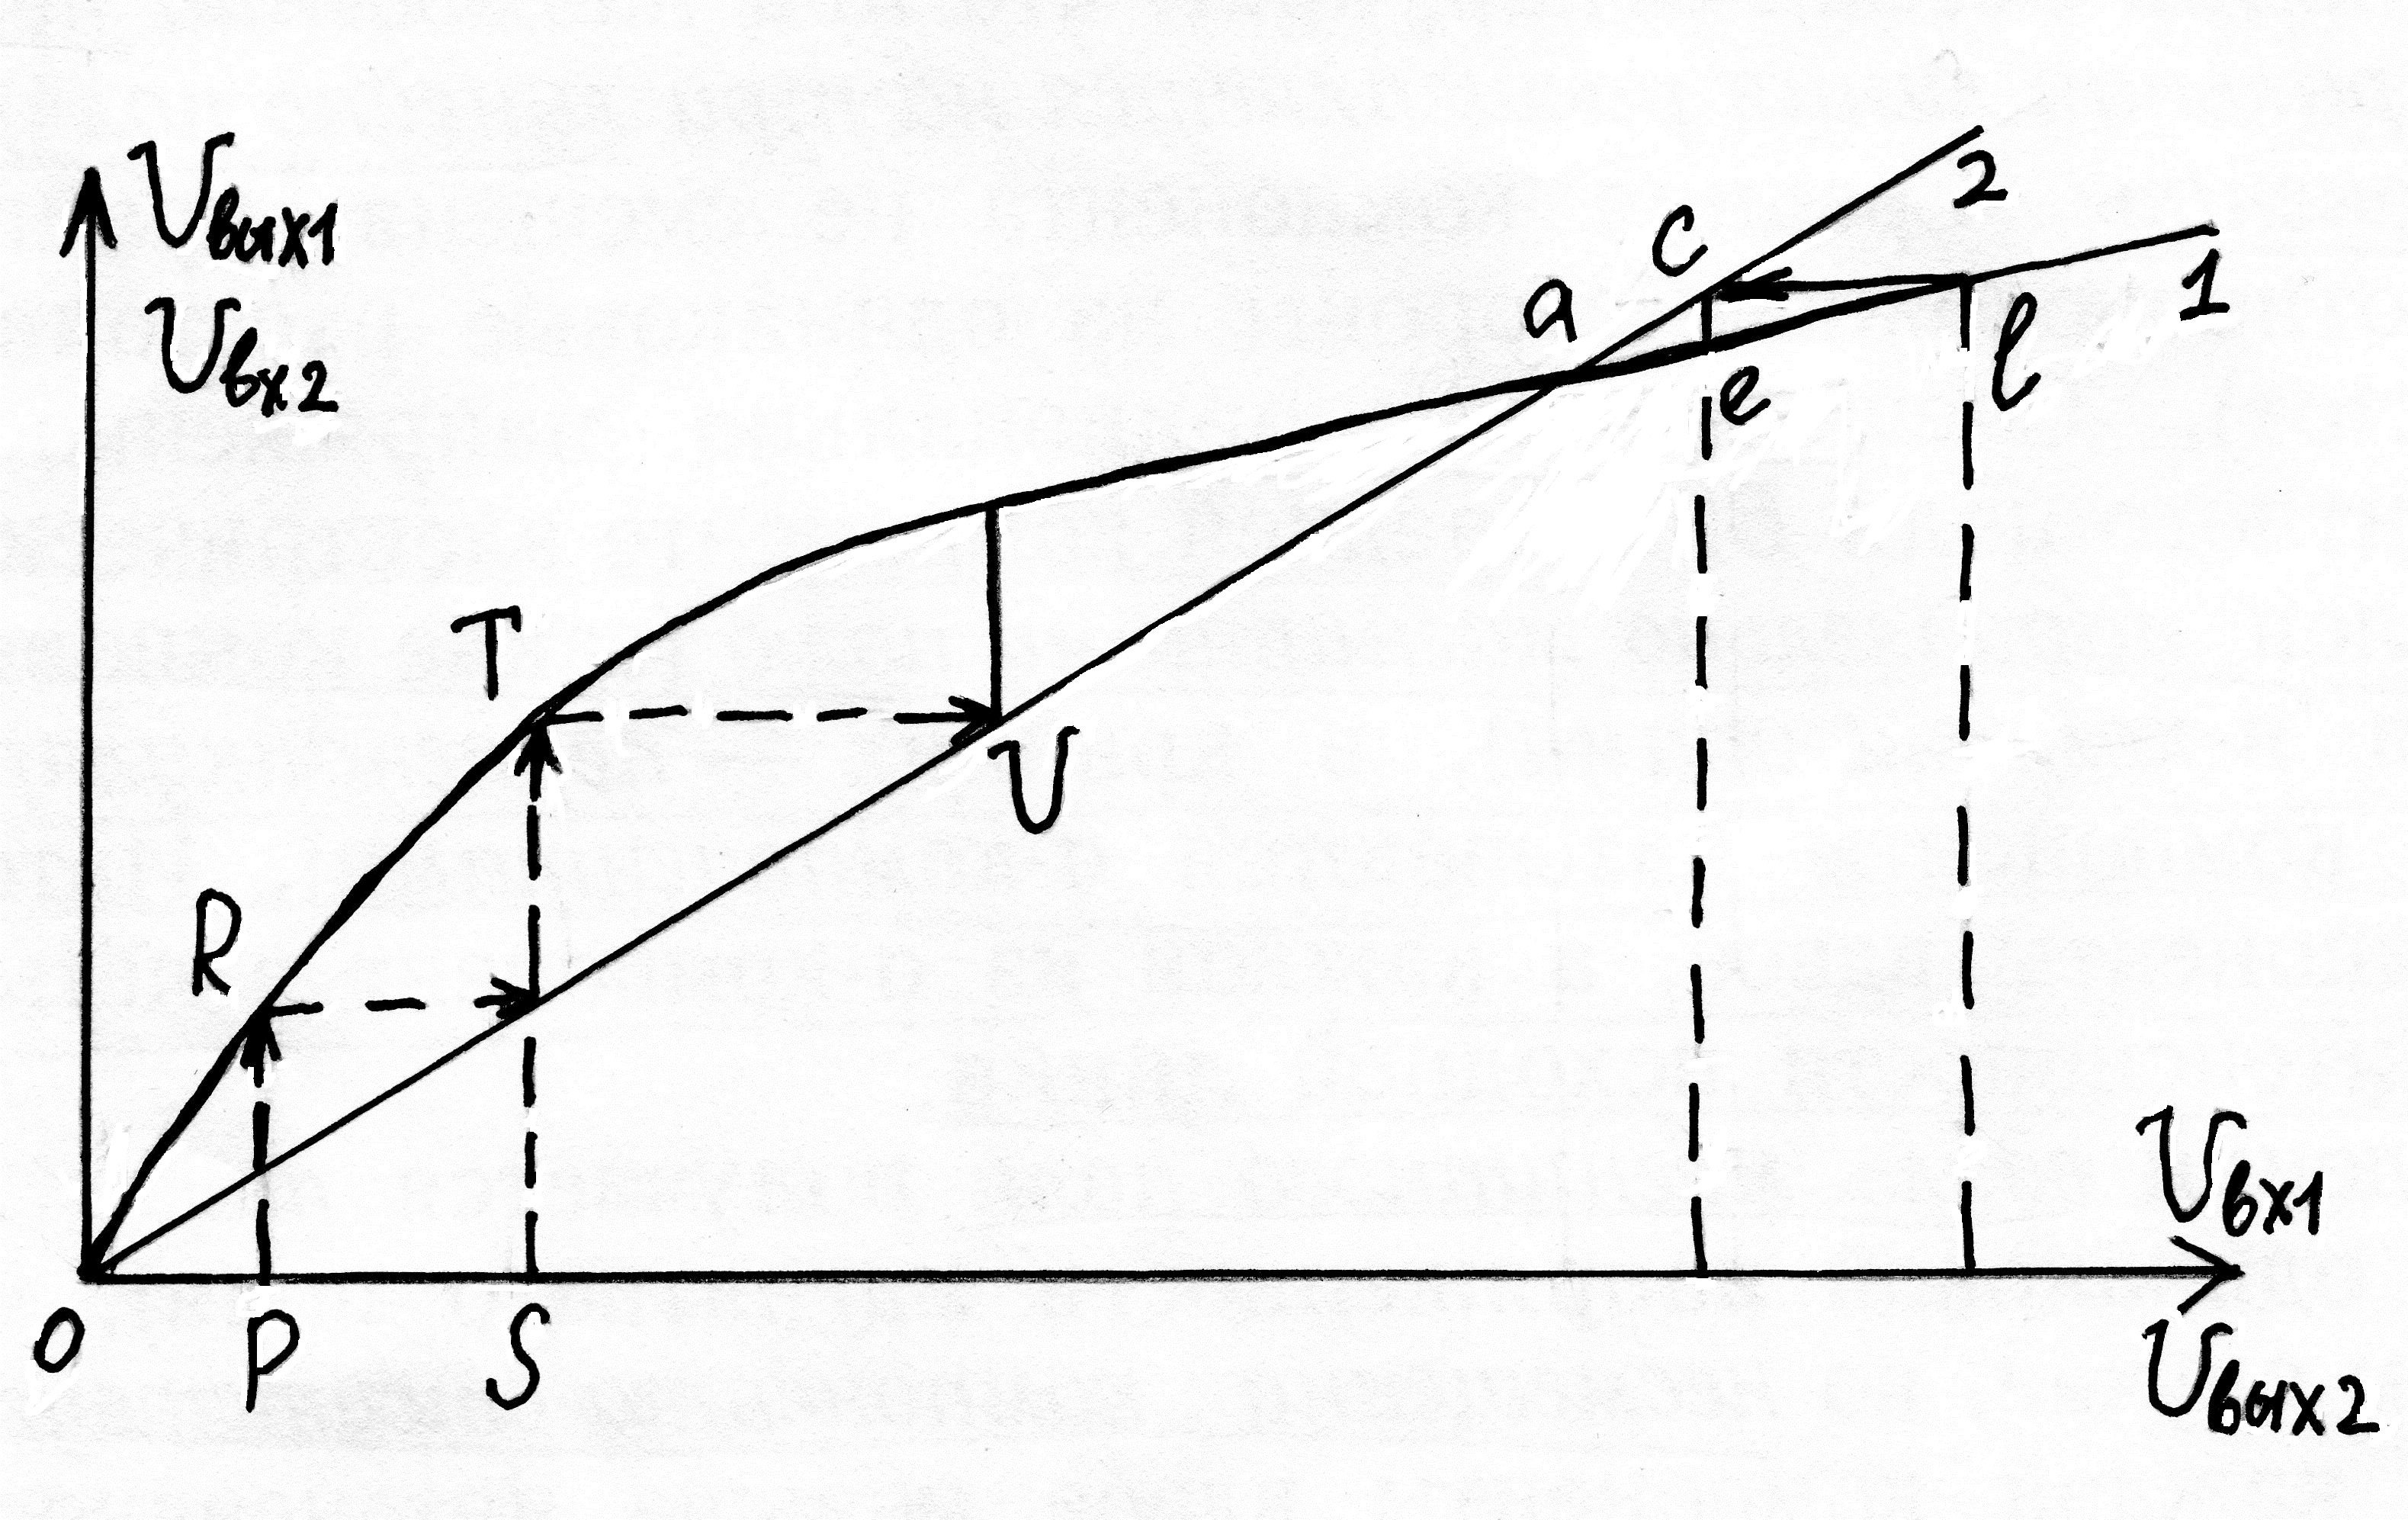
\includegraphics[width=0.4\linewidth]{circuit/fig8}
	\caption{}
	\label{fig:fig8}
\end{figure}

Отметим, что точка $O$ тоже удовлетворяет условию \eqref{eq:7} и соответствует второму стационарному состоянию. Убедимся, что точка $\alpha$ соответствует устойчивому стационарному состоянию, а точка $O$ - неустойчивому.

Пусть схема находится в точке $O$. Если флуктуация приведет к амплитуде $Р$ напряжения база-эмиттер, то амплитуда напряжения на контуре будет $R$: по обратной связи это вызовет увеличение амплитуды напряжения база-эмиттер до величины $S$, что, в свою очередь, вызовет переход в точку $T$ и т.д., пока схема не придет к точке $\alpha$.

Проведем аналогичные рассуждения относительно состояния в точке $\alpha$. Пусть флуктуация выведет амплитуду напряжения на контуре из точки $\alpha$ в точку $b$. Через обратную связь (через точку $c$) это вызовет амплитуду напряжения база-эмиттер величиной $d$, но ей будет соответствовать амплитуда $e$ напряжения на контуре. Другими словами, схема вернется в состояние $\alpha$, что и доказывает устойчивость этого состояния.

Совершенно аналогичным путем легко доказать устойчивость состояний $O$ и $\alpha$ и неустойчивость состояния $b$ для схемы, имеющей иной вид колебательной характеристики (рис.\ref{fig:fig9}).

\begin{figure}[h]
	\centering
	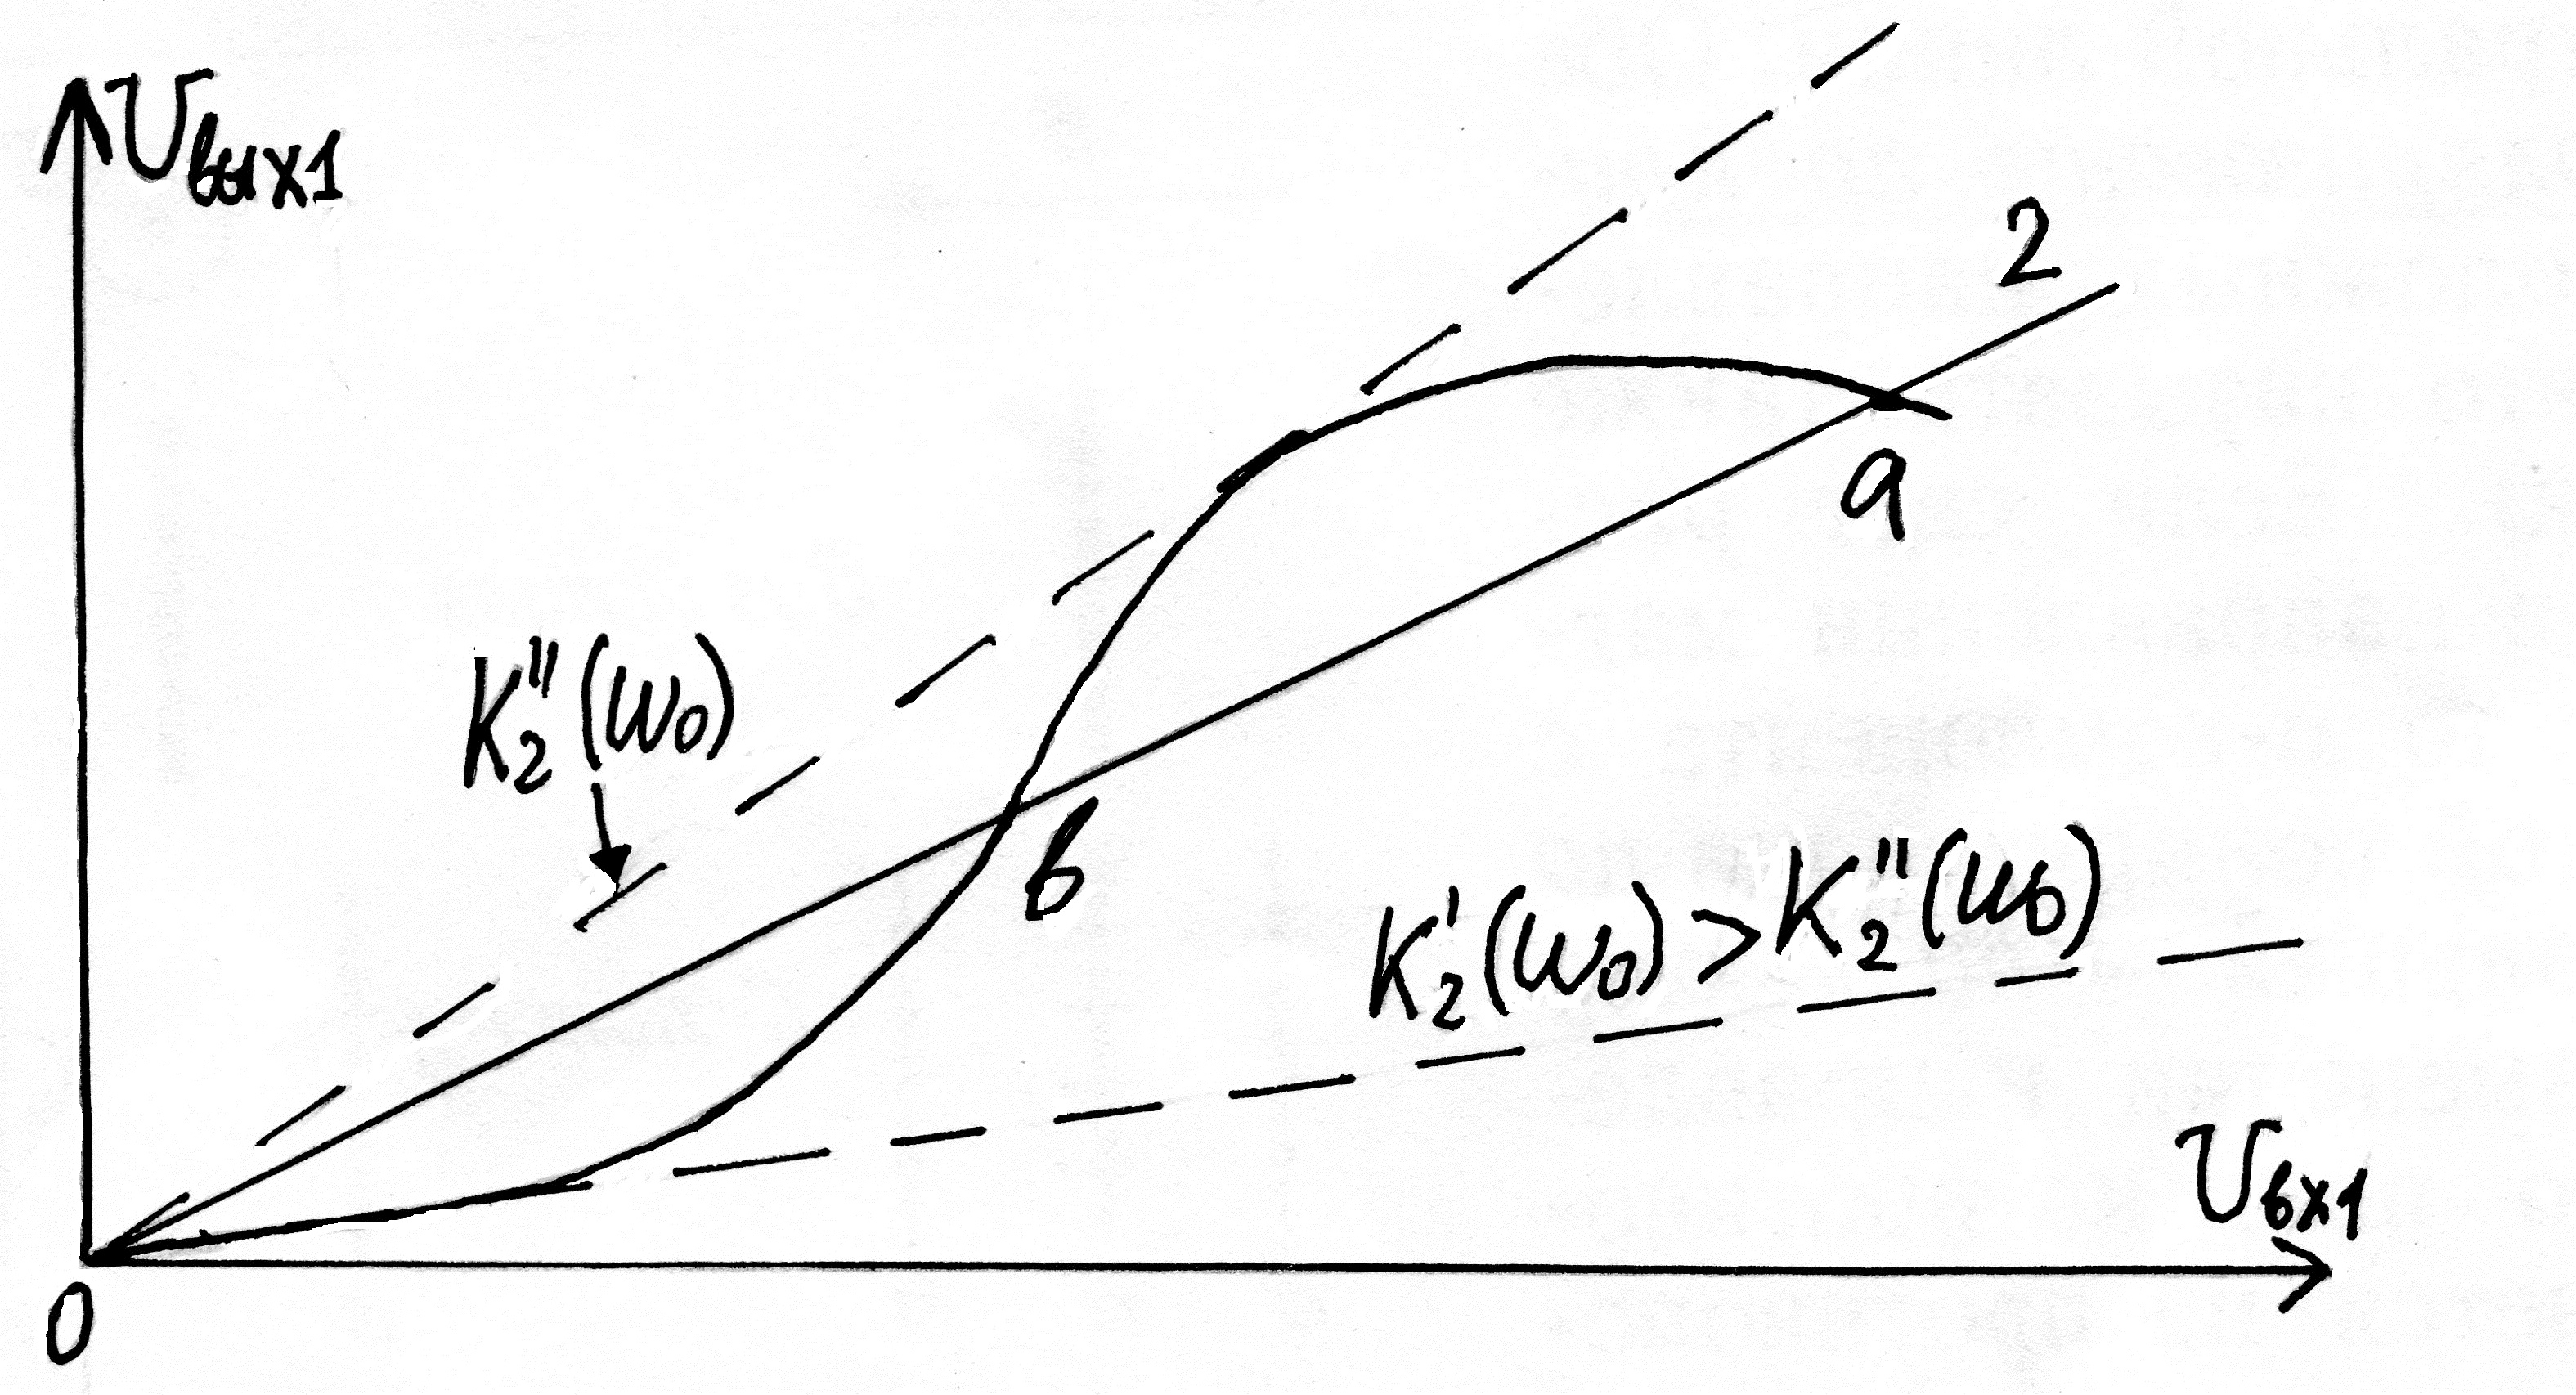
\includegraphics[width=0.4\linewidth]{circuit/fig9}
	\caption{}
	\label{fig:fig9}
\end{figure}

Режим возбуждения автогенератора, проиллюстрированный рис.\ref{fig:fig8}, называют мягким, режим, соответствующий рис.\ref{fig:fig9} - жестким режимом возбуждения. Различие между мягким и жестким режимами возбуждения, выявляемое при сравнении рис.\ref{fig:fig8} и рис.\ref{fig:fig9}, наглядно прослеживается и в характере зависимости амплитуды стационарных колебаний от степени связи, т.е. от величины $K_2(\omega_0)$ представленной на рис.\ref{fig:fig10} для мягкого режима и на рис.\ref{fig:fig11} - для жесткого.

\begin{center}
    \begin{minipage}{0.49\linewidth}
        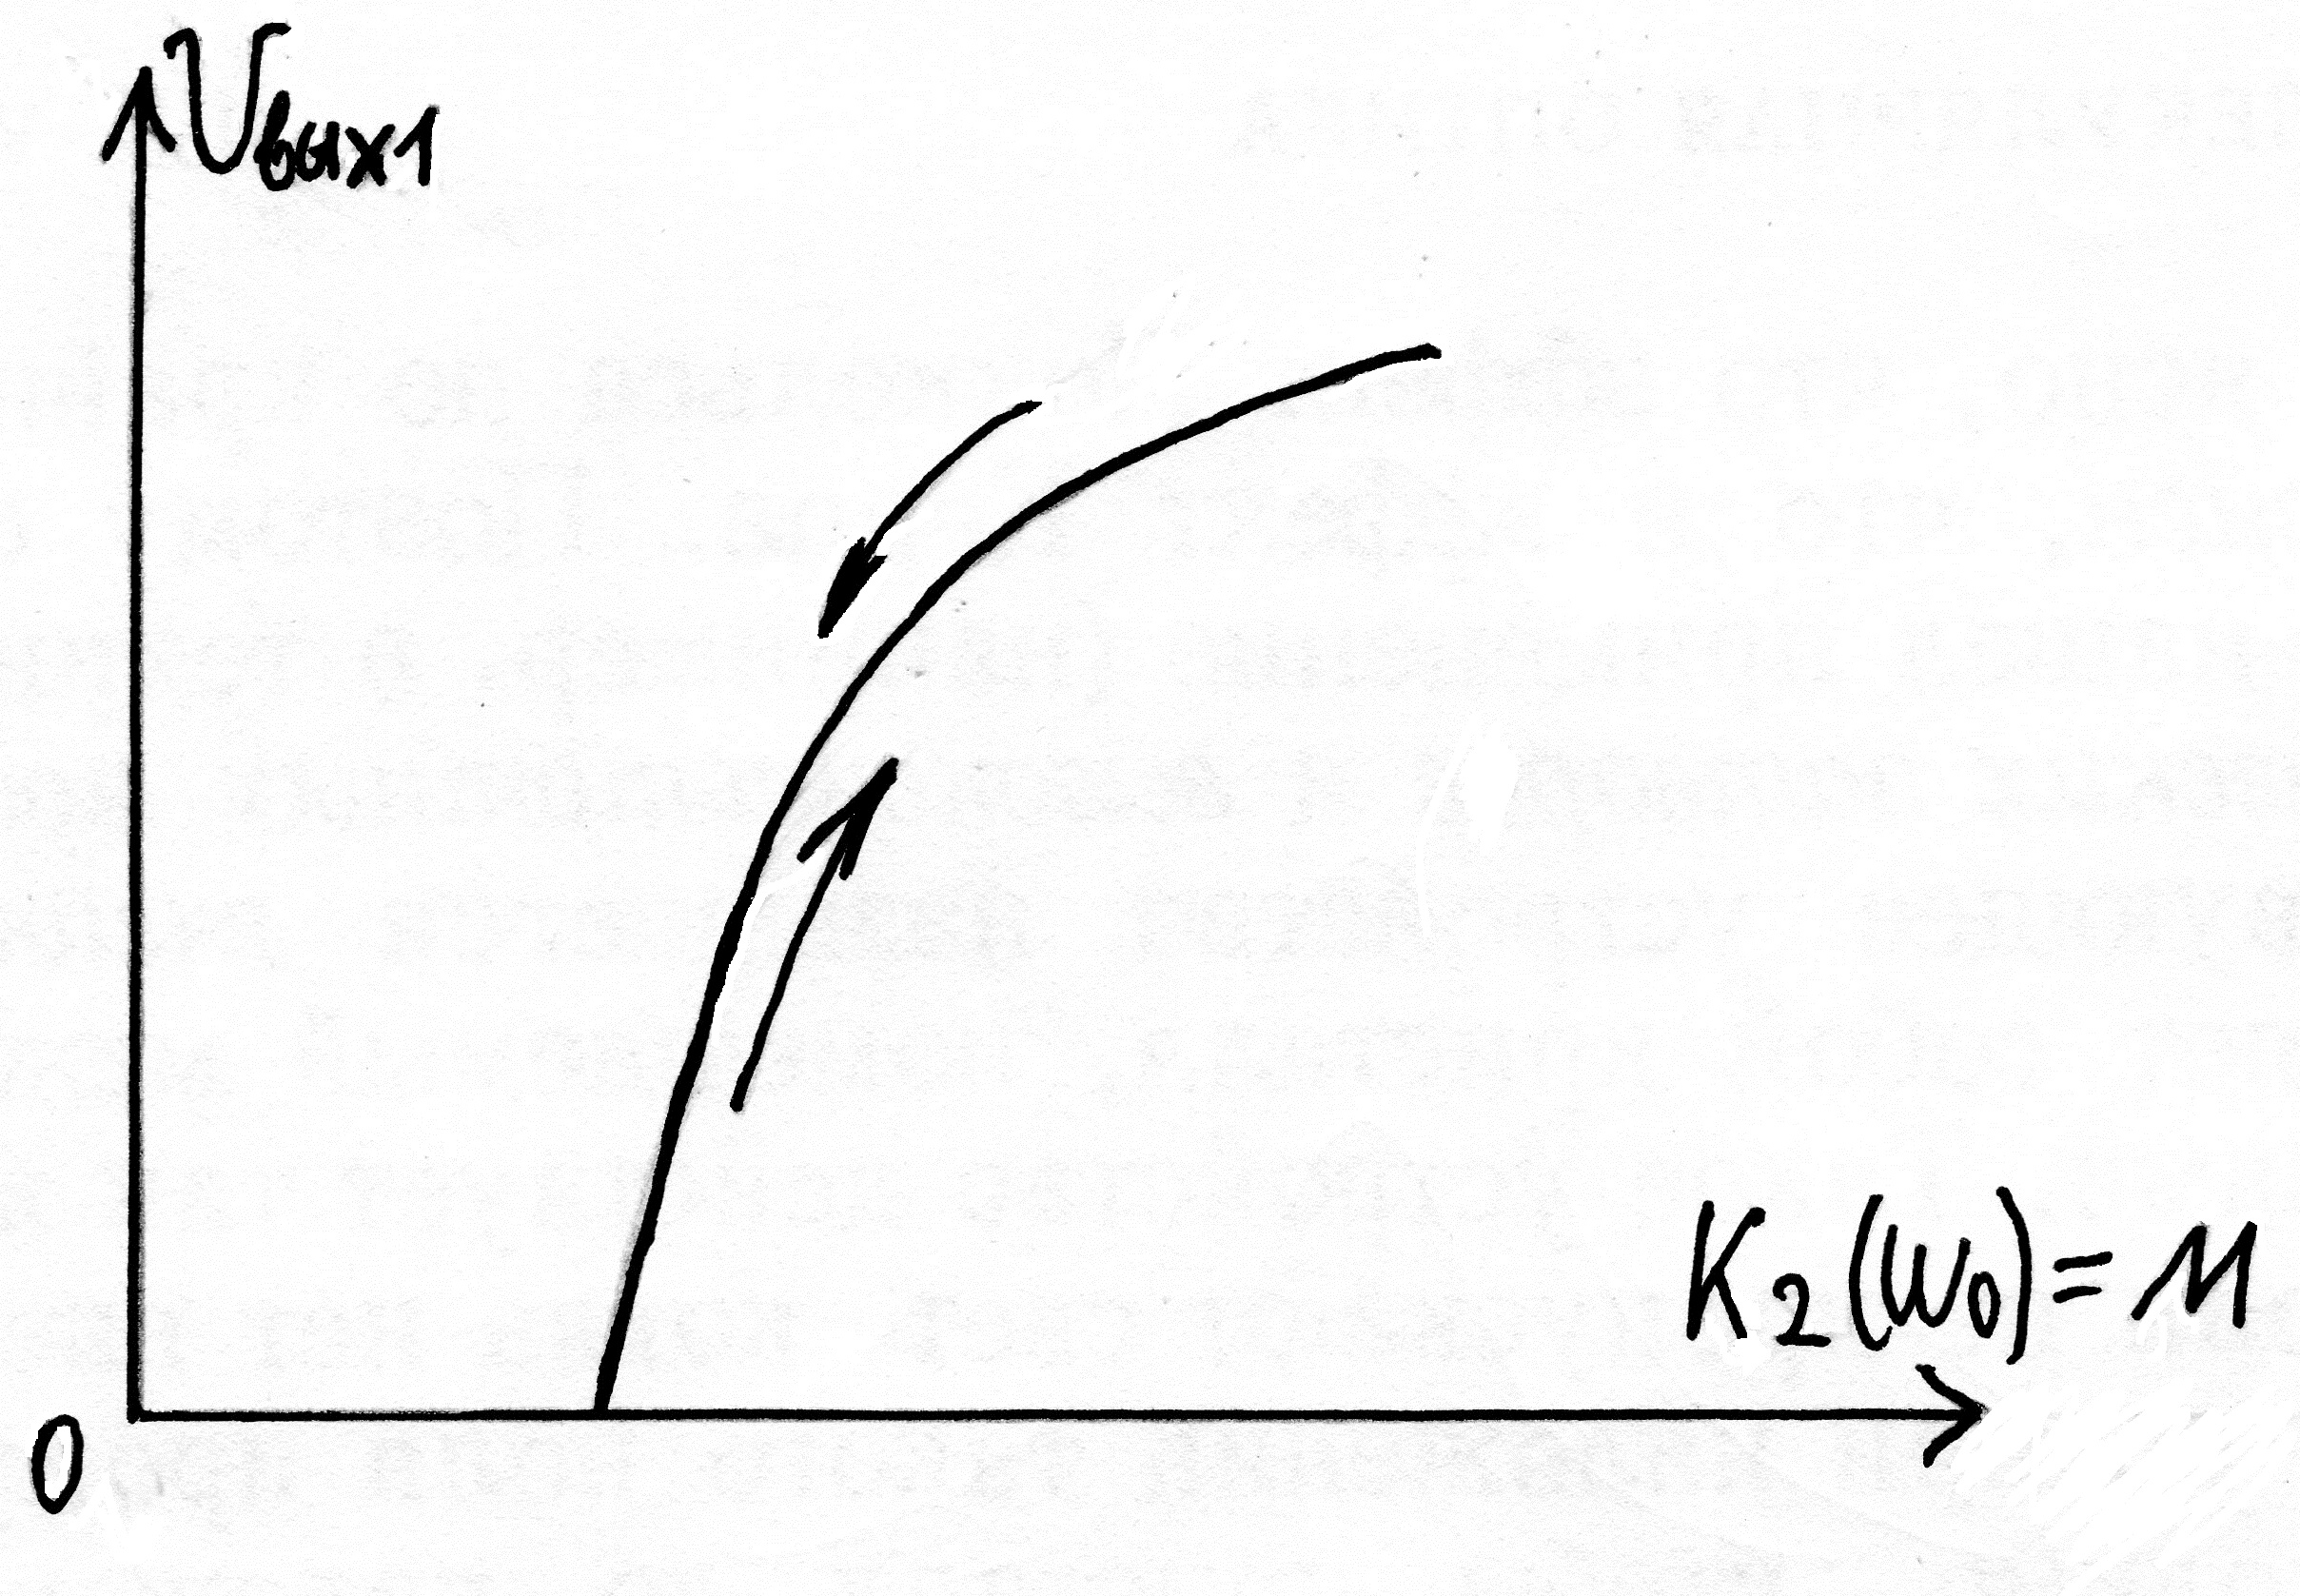
\includegraphics[width=\linewidth]{circuit/fig10} 
        \label{fig:fig:10}
        \captionof{figure}{} 
    \end{minipage}
\hfill     
    \begin{minipage}{0.49\linewidth}
        \centering
        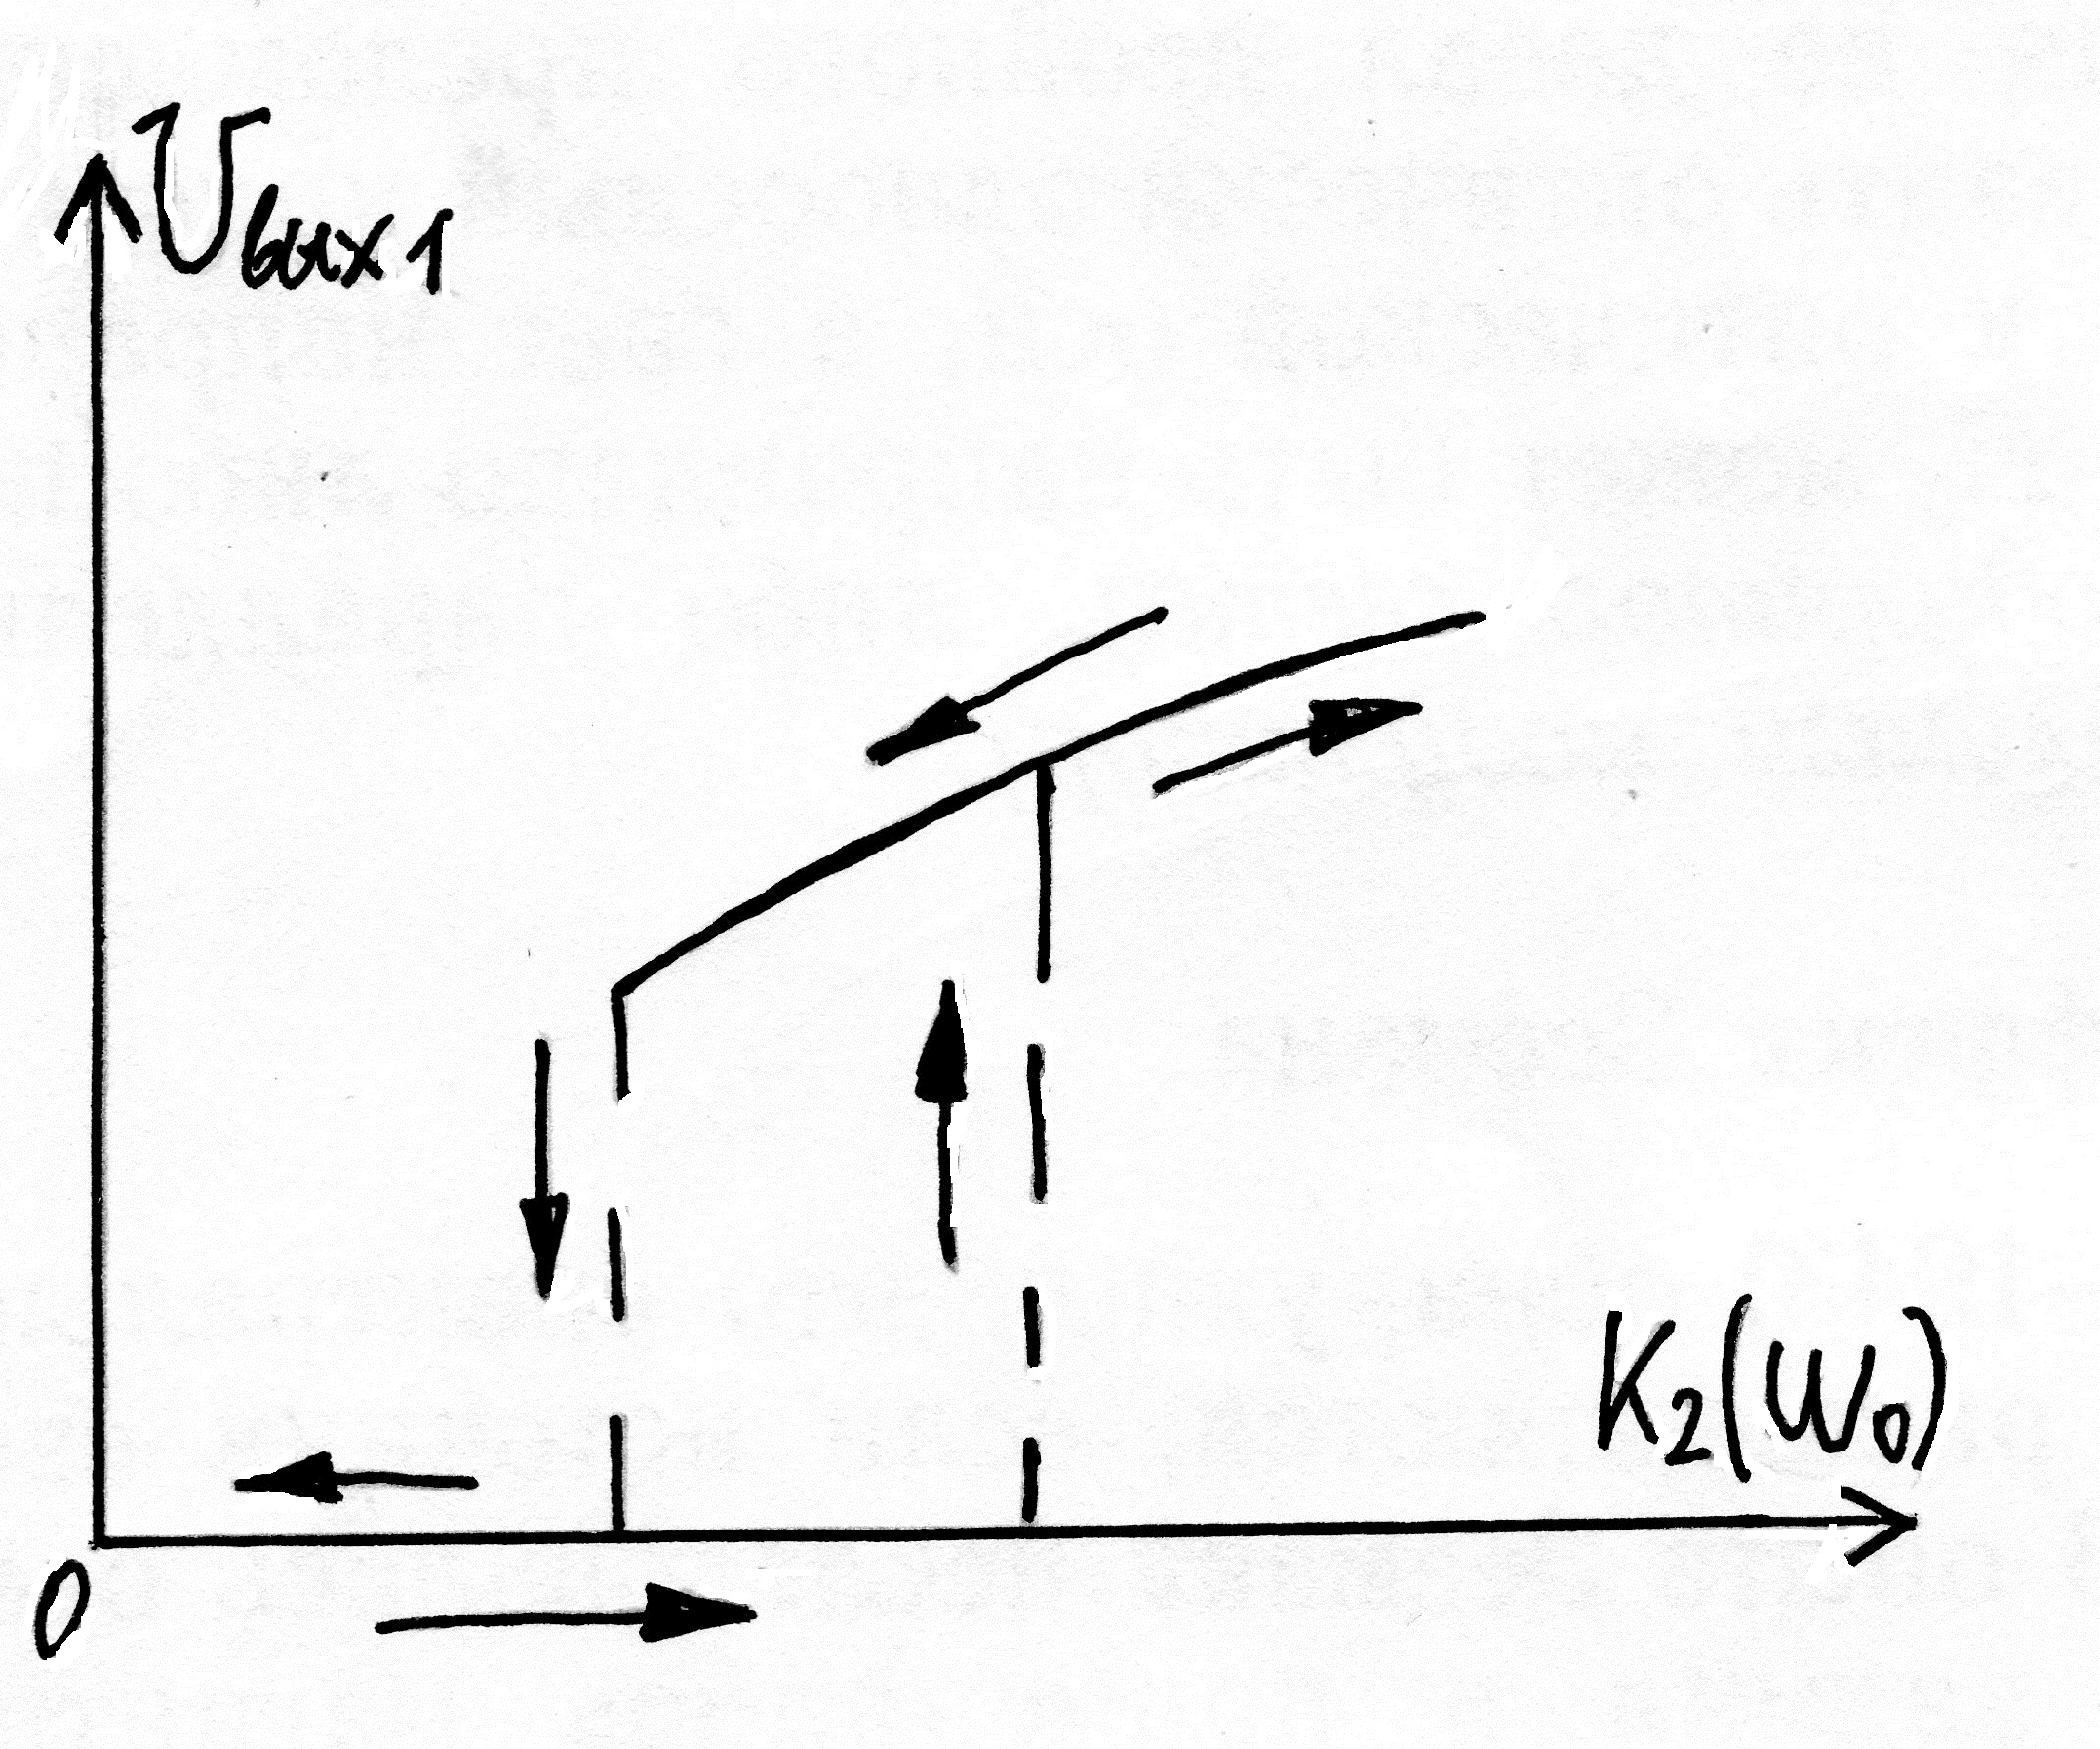
\includegraphics[width=\linewidth]{circuit/fig11}  
        \label{fig:fig:11}
        \captionof{figure}{} 
    \end{minipage} 
\end{center} 

Наличие петли гистерезиса на рис.\ref{fig:fig11} объясняется тем, что колебания возникают при связи, большей, чем связь, при которой происходит срыв колебаний. Это обстоятельство становится ясным из рис.\ref{fig:fig9}: колебания возбуждаются при связи $K'_2(\omega_0)$, а срываются при $K''_2(\omega_0)<K'_2(\omega_0)$.

Следует заметить, что для возникновения колебаний в автогенераторе с жестким режимом возбуждения необходим внешний толчок, достаточный, чтобы вывести схему вверх через порог, задаваемый точкой $b$ (см.рис.\ref{fig:fig9}).

\section{Анализ схемы автогенератора}

Существует множество различных вариантов технической реализации автогенератора.

Простейшая схема автогенератора с индуктивной обратной связью, где в качестве усилительного элемента использован транзистор, приведена на рис.\ref{fig:fig2}. Здесь избирательность по частоте обеспечивается параллельным колебательным контуром, включенным в коллекторную цепь транзистора $T$.

Колебательный контур, собственные потери которого характеризуются сопротивлением $r$, на резонансной частоте $\omega_0=1/{LC}$ имеет сопротивление $R=\rho^2/r$, где $\rho=\sqrt{L/C}$. Добротность контура $Q=\rho/r\gg1$

Для анализа процессов, происходящих в генераторе, воспользуемся его эквивалентной схемой по переменному току, изображенной на риc.\ref{fig:fig12}.

% \begin{wrapfigure}{l}{0.4\linewidth}
% 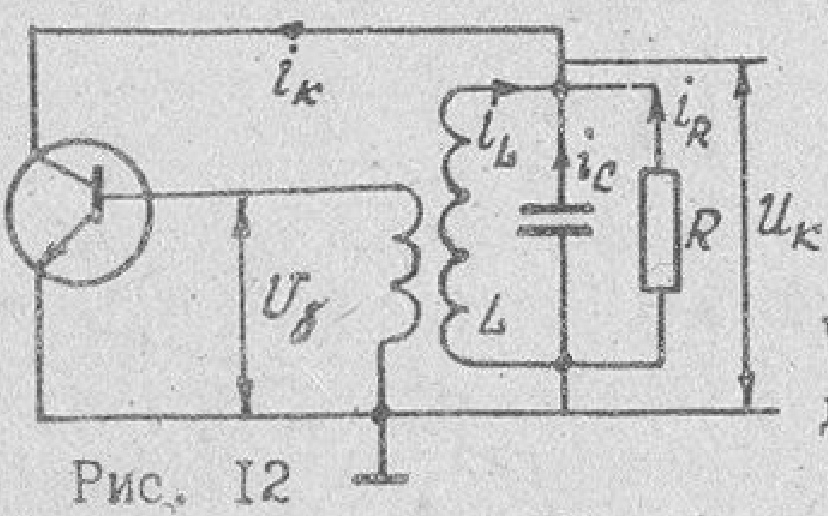
\includegraphics[width=\linewidth]{circuit/12.jpg}
% \caption{}
% \label{fig:fige12}
% \vspace{-20pt}
% \end{wrapfigure}
\begin{figure}[h]
	\centering
	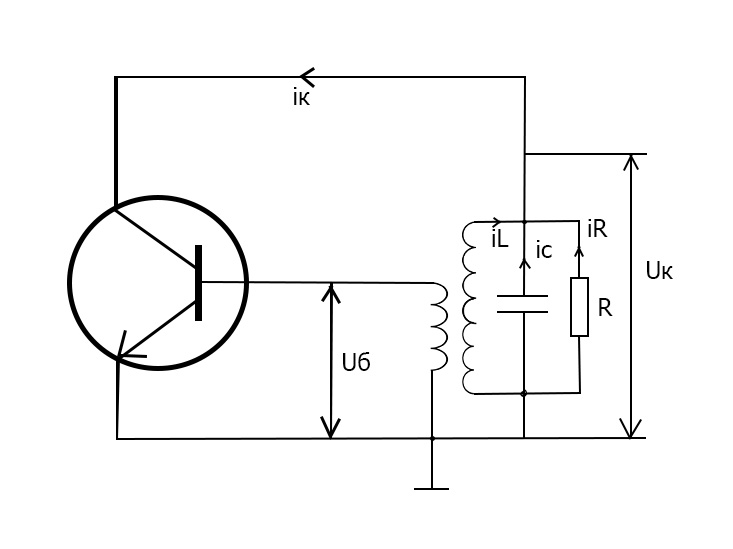
\includegraphics[width=0.7\linewidth]{circuit/fig12}
	\caption{}
	\label{fig:fig12}
\end{figure}

Коллекторный ток
\begin{equation*}
\begin{aligned}
&i_k=i_C+i_R+i_L \\
&i_C=C\frac{\operatorname dU_k}{\operatorname dt} \\
&i_L=\frac{1}{L}\int U_k \operatorname dt \\
&i_r=\frac{U_k}{R}
\end{aligned}
\end{equation*}
- соответственно ток через емкость, сопротивление и индуктивность колебательного контура.

Если рассматривать ту область частот,где инерционными свойствами транзистора, т.е. зависимостью его параметров от частоты,можно пренебречь,то ток коллектора в зависимости от напряжений на базе $U_\text{б}$ на коллекторе $U_k$ транзистора можно представить в виде функции $i_k(t)=i_k(U_\text{б}(t),U_k(t))$. Приемлимой аппроксимацией является представление этой функции в виде $i_k=i_k(U_\text{б}-DU_k)$, когда $i_k$ зависит не от каждого из напряжений $U_\text{б}$ и $U_k$ в отдельности, а от управляющего напряжения $U_\text{упр}=U_\text{б}-DU_k$. Параметр $D$, называемый проницаемостью, характеризует влияние коллекторного напряжения на выходной ток транзистора. С учетом сказанного выше
\begin{equation}
i_k=i_k(U_\text{б}-DU_k)=C\frac{\operatorname dU_k}{\operatorname dt}+\frac{U_k}{R}+\frac{1}{L}\int U_k \operatorname dt
\label{eq:8}
\end{equation}{}

В пренебрежении током базы напряжение $\displaystyle U_\text{б}=М\frac{\operatorname di_L}{\operatorname dt}$, а $\displaystyle U_k=L\frac{\operatorname di_L}{\operatorname dt}$. Отсюда следует, что $U_\text{упр}=U_\text{б}-DU_k=(M/L-D)U_k=\varkappa U_k$. Продифференцировав \eqref{eq:8} по времени, получаем следующее нелинейное дифференциальное уравнение
\begin{equation}
\frac{\operatorname d^2U_k}{\operatorname dt^2}+\frac{\operatorname d}{\operatorname dt}[\frac{U_k}{CR}-\frac{1}{C}i_k(\varkappa U_k)]+\omega_0^2U_k=0
\label{eq:9}
\end{equation}

Для его решения необходимо знать конкретную зависимость $i_k(\varkappa U_k)$, которая выше описана степенным полиномом \eqref{eq:2}. 

При отсутствии внешних возмущений колебания в генераторе возникнут, когда будут выполнены условия его самовозбуждения. В этом случае выходное напряжение сначала будет нарастать со временем, а
затем выйдет на стационарный уровень с постоянной амплитудой $U_\text{ст}$ (рис.\ref{fig:figure13}). Найдем
\begin{enumerate}
\item условия возникновения колебаний в автогенераторе
\item стационарную амплитуду автоколебаний.
\end{enumerate}

\begin{wrapfigure}{l}{0.4\linewidth}
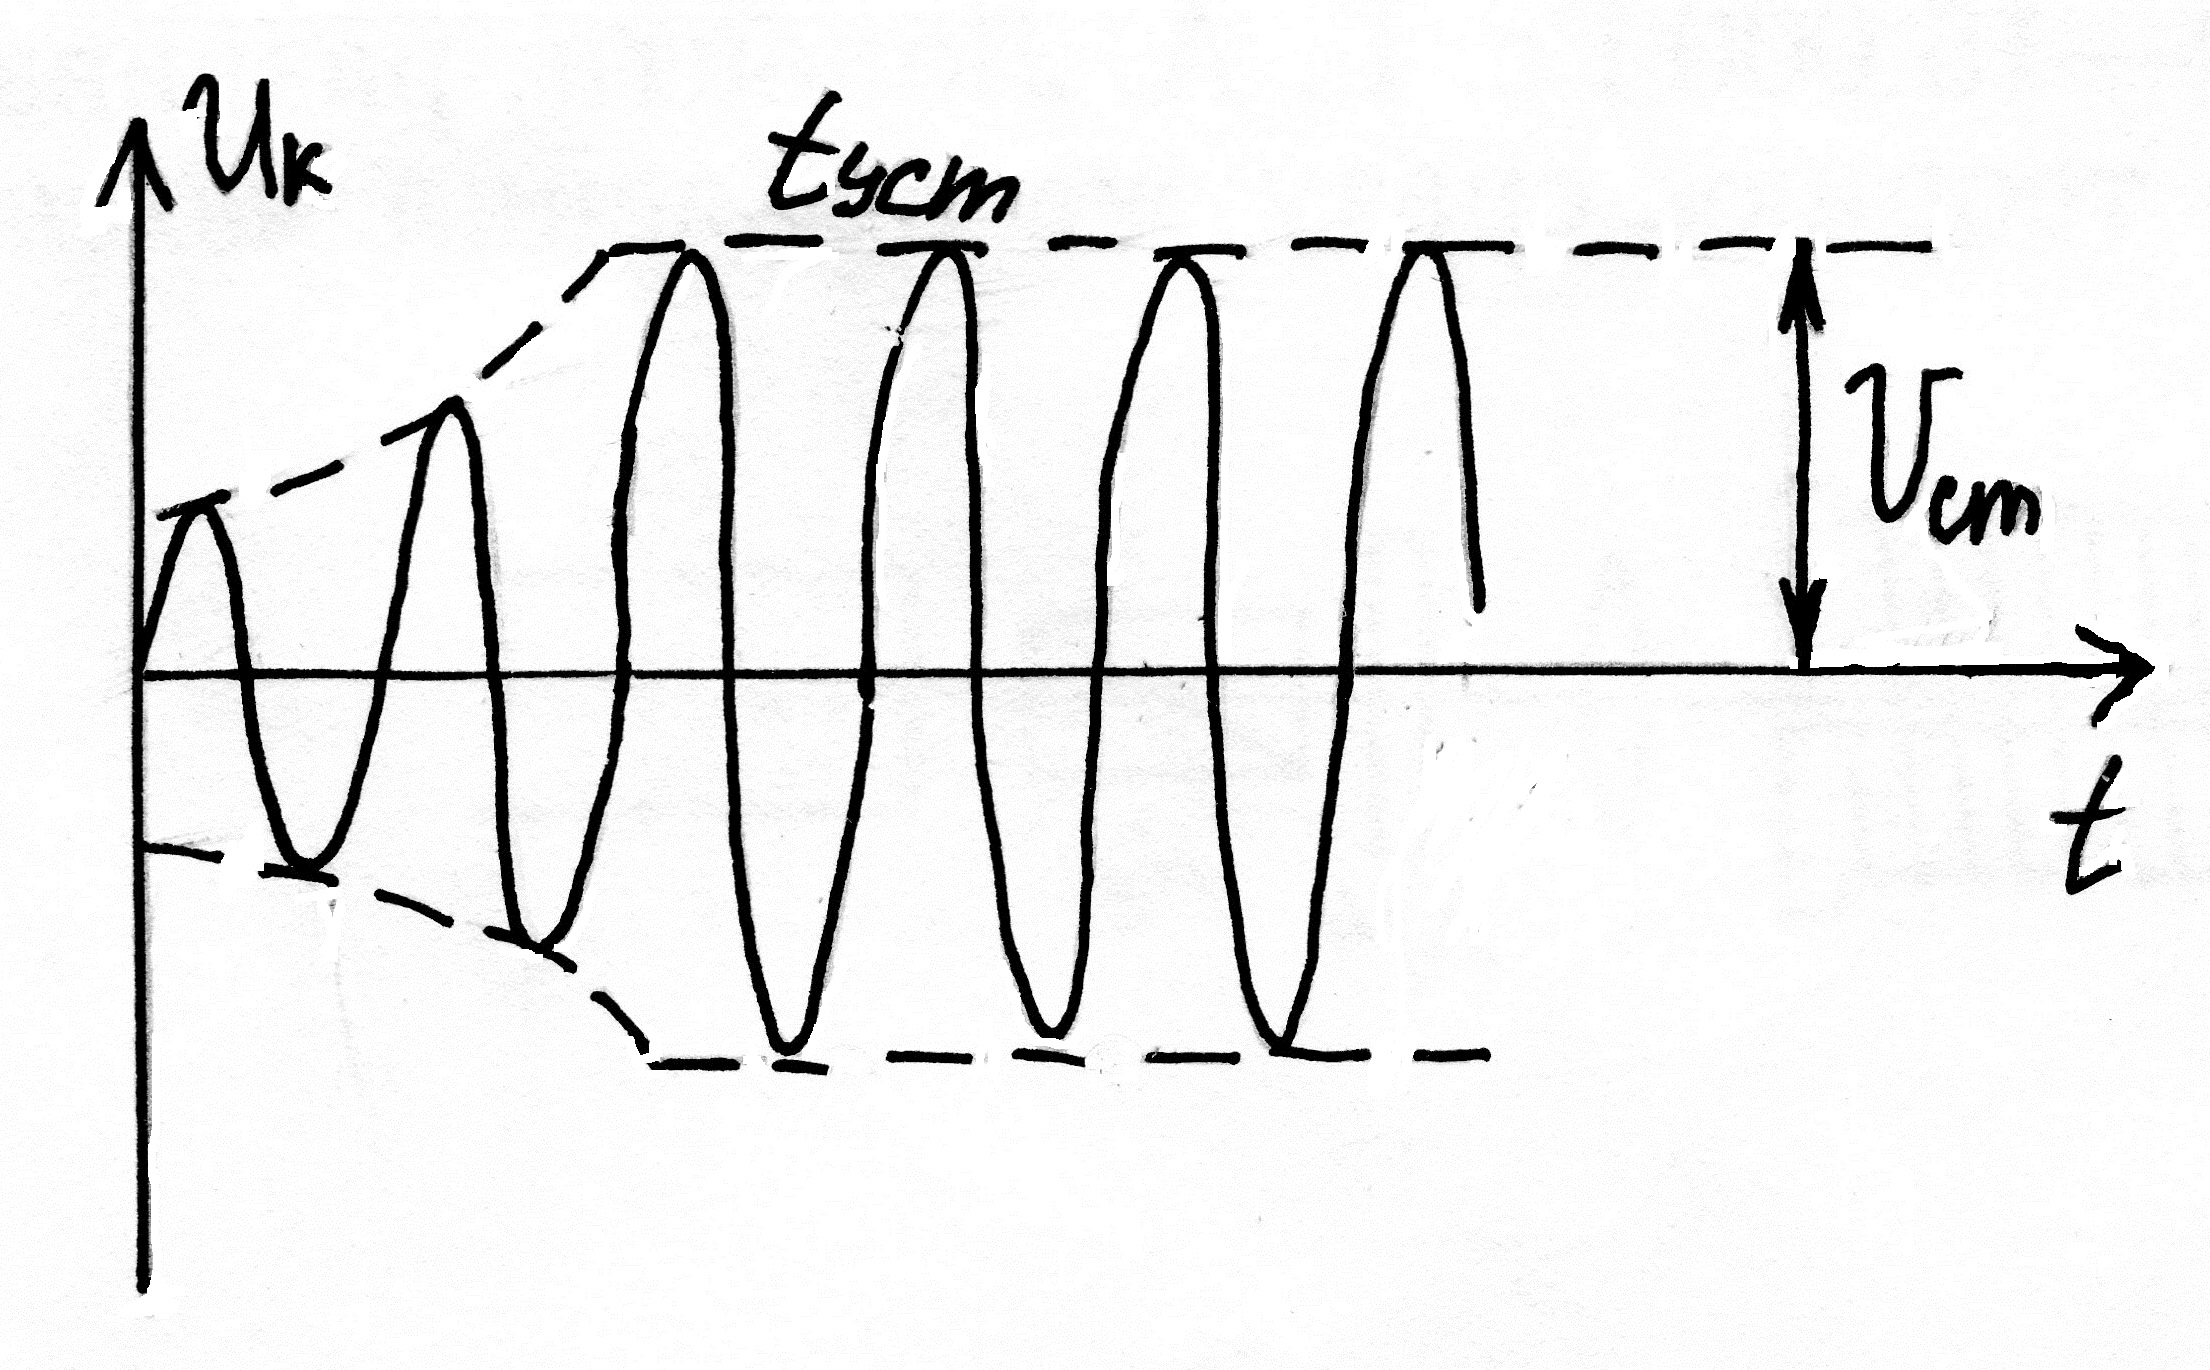
\includegraphics[width=\linewidth]{circuit/fig13}
\caption{}
\label{fig:figure13}
\vspace{-20pt}
\end{wrapfigure}

Рассмотрим начальную стадию процесса генерации для времен много меньших времени установления колебаний $t_\text{уст}$. В этом случае уровень колебаний незначителен и транзистор находится в линейном режиме. В разложении $i_k=i_k(\varkappa U_k)$ по степеням $\varkappa U_k$ отличным от нуля будет лишь коэффициент $b_1=S_0$, остальные $b_n=0$ ($n\gg2$).

Тогда вместо уравнения \eqref{eq:9} получаем линейное дифференциальное уравнение с постоянными коэффициентами

\begin{equation}
\frac{\operatorname d^2U_k}{\operatorname dt^2}+2\alpha \frac{\operatorname d U_k}{\operatorname dt}+\omega_0^2U_k=0
\label{eq:10}
\end{equation}
в котором

\begin{equation}
2\alpha=\frac{1}{L}(r+\frac{\rho^2}{r_k^*}-\frac{S_0M}{C})
\label{eq:11}
\end{equation}
$\displaystyle r=\rho^2/R$ - собственное активное сопротивление колебательного контура, $\displaystyle \rho^2/r_k^*=r_\text{вн}$ - внесенное в контур сопротивление за счет шунтирующего действия на него внутреннего сопротивления транзистора $r_k^*$; $-S_0M/C=r_{-}$ - добавочное сопротивление, вносимое в контур за счет обратной связи. 

Общее решение уравнения \eqref{eq:10}
\begin{equation*}
U_k=A_0\exp(-\alpha t)\cos(\omega_\text{св}t+\phi_0)
\end{equation*}
где $A_0$ и $\phi_0$ - постоянные, зависящие от начальных условий, $\omega_\text{св}=\sqrt{\omega_0^2-\alpha^2}$ - частота колебаний. Так как добротность $Q\gg1$, то $\alpha^2\ll \omega_0^2$ и $\omega_\text{св}\approx\omega_0^2$

Амплитуда колебаний со временем будет расти, если $\alpha<0$ или 
\begin{equation}
\frac{S_0M}{rC}>1+\frac{\rho^2}{r\cdot r_k^*}=1+\frac{R}{r_k^*}
\label{eq:12}
\end{equation}

Выполнение неравенства \eqref{eq:12} означает, что автогенератор является неустойчивой системой. По этому признаку \eqref{eq:12} есть условие самовозбуждения. Оно будет выполнено, если:
\begin{enumerate}
\item обратная связь положительна - коэффициент взаимоиндукции $M$ имеет такой знак, что сдвиг фазы между напряжениями коллектор-эмиттер и база-эмиттер равен $180^{\circ} (r_{-}<0)$;
\item обратная связь достаточно глубокая - энергия, вносимая в контур, превышает энергию потерь ($|r_{-}|>r+r_\text{вн}$). Частота генерации $\omega_\text{г}\simeq\omega_0$
\end{enumerate}

Если сопротивлени коллекторного перехода $r_k^*\gg R$ - резонансного сопротивления, то условие самовозбуждения будет иметь более простой вид:
\begin{equation}
\frac{S_0M}{rC}>1
\label{eq:13}
\end{equation}

Перепишем левую часть \eqref{eq:13} в ином виде:
\begin{equation*}
\frac{S_0M}{rC}=S_0\frac{1}{r}\frac{L}{C}\frac{M}{L}=(S_0R)n=K_1K_2,
\end{equation*}
где $K_1$ - коэффициент усиления резонансного усилителя; $n=K_2$ - коэффициент передачи трансформатора L\textdiv $L_\text{св}$

Очевидно, что \eqref{eq:13} совпадает с условием \eqref{eq:1}.

Нарастание колебаний происходит за время $t_\text{уст}\gg 2\pi / \omega_0$. Поэтому генерируемое напряжение почти синусоидально в каждый из текущих моментов времени $t$ от начала генерации до ее установления, т.к. амплитуда и фаза колебаний являются медленными функциями времени. С учетом зависимости параметров транзистора от амплитуды в соответствии с квазилинейным методом $S_0$ нужно заменить на $S_\text{ср}$, а $r_k^*$ на $R'_i$. Тогда вместо \eqref{eq:9} будем иметь уравнение 

\begin{equation}
\frac{\operatorname d^2U_k}{\operatorname dt^2}-2\alpha_\text{ср} \frac{\operatorname d U_k}{\operatorname dt}+\omega_0^2U_k=0
\label{eq:14}
\end{equation}
где 
\begin{equation}
2\alpha_\text{ср} = \frac{1}{L}(r+\frac{\rho^2}{R'_i}-\frac{S_\text{ср}M}{C})
\label{eq:15}
\end{equation}

В стационарном режиме $U_k=\text{const}$. Следовательно, постоянны и $R'_i$ и $S_\text{ср}$. Форма напряжения на контуре синусоидальна, что можно представить как результат решения уравнения для гармонического осциллятора
\begin{equation}
\frac{\operatorname d^2U_k}{\operatorname dt^2}+\omega_0^2U_k=0
\label{eq:16}
\end{equation}
Уравнения \eqref{eq:14} переходит в \eqref{eq:16}, если $\alpha_\text{ср}=0$, или
\begin{equation*}
\frac{S_\text{ср}M}{rC}=1+\frac{R}{R'_i}
\end{equation*}

Полученное равенство определяет амплитуду стационарных колебаний и называется условием баланса амплитуд. Смысл его в том, что в стационарном режиме вносимая в контур энергия равна энергии потерь. Вносимая энергия характеризуется средним добавочным сопротивлением $r^\text{ср}_{-}=-S_\text{ср}M/C$, а энергия потерь - суммой $r+r^\text{ср}_{\text{вн}1}=r+\rho^2/R'_i$. В установившемся режиме $|r^\text{ср}_{-}|=r+r^\text{ср}_\text{вн}$.

Если реакция коллекторного напряжения незначительна $R'_i\gg R$, то условием баланса амплитуд будет
\begin{equation}
\frac{S_\text{ср}M}{Cr}=1
\label{eq:17}
\end{equation}

Отметим, что поскольку величина $S_\text{ср}R$ является коэффициентом усиления по первой гармонике $K_1$ нелинейного резонансного усилителя, то \eqref{eq:17} можно записать в виде
\begin{equation*}
K_1K_2=1
\end{equation*}
что совпадает с \eqref{eq:7}.

Из соотношения \eqref{eq:17}, используя экспериментальную зависимость $S_\text{ср}$ от амплитуды колебания на базе транзистора (см.рис.\ref{fig:fig5}), можно найти стационарную амплитуду этого колебания.

Значение стационарной амплитуды колебаний можно найти и с помощью колебательной характеристики. Действительно, с учетом \eqref{eq:4} условие $K_1K_2=1$ равносильно соотношению
\begin{equation*}
\frac{I_1(U_\text{б})}{U_\text{б}}RK_2=1
\end{equation*}
или
\begin{equation}
I_1(U_\text{б})=U_\text{б}\frac{1}{RK_2}
\label{eq:18}
\end{equation}
Используя экспериментальные зависимости (см.рис\ref{fig:fig6}) и графически отыскивая решение уравнения \eqref{eq:18} относительно $U_\text{б}$, получим искомое значение стационарной амплитуды.

\section{Описание лабораторного макета}

\begin{wrapfigure}{l}{0.4\linewidth}
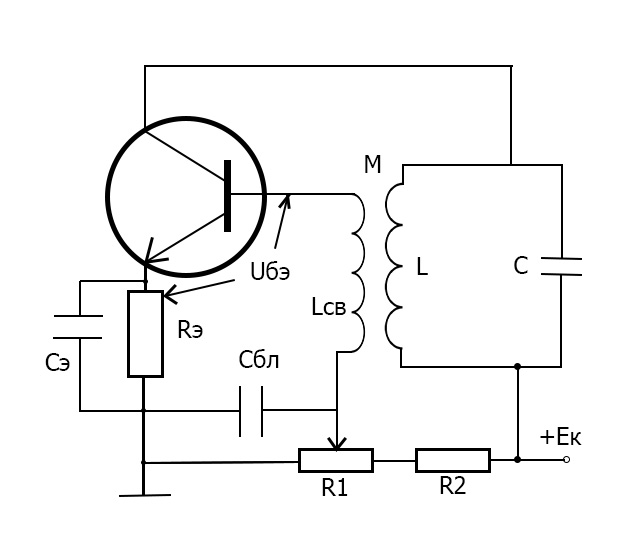
\includegraphics[width=\linewidth]{circuit/fig14}
\caption{}
\label{fig:fig14}
\vspace{-17pt}
\end{wrapfigure}

Обычно автогенератор питают не от двух источников, как это изображено на рис.\ref{fig:fig2}, а от одного. Поэтому экспериментально в данной лабораторной работе будет исследоваться генератор, выполненный по схеме, изображенной на рис.\ref{fig:fig14}. В качестве усилительного элемента используется кремниевый $n-p-n$ транзистор КТ306 Б. Его начальный режим но постоянному току обеспечивается резисторами $R_\text{э}, R_1$ и $R_2$. Напряжение, снимаемое с $R_1$ может плавно изменяться, что позволяет изменять начальное напряжение смещения на базе $E_\text{см}$ (по отношению к эмиттеру). Емкость $C_\text{бл}$	- блокировочная и служит для того, чтобы отфильтровать переменную составляющую напряжения, снимаемого с потенциометра $R_1$. Сопротивление $R_\text{э}$ - элемент термостабилизации начальной рабочей точки. Емкость $C_\text{э}$ отфильтровывает переменную составляющую, напряжения на $R_\text{э}$, если $1/\omega_0 C_\text{э}\ll R_\text{э}$, и обеспечивает таким образом "заземление" эмиттера по переменному току. В результате транзистор оказывается включенным по схеме с общим эмиттером.

Помимо этого цепочка $R_\text{э}C_\text{э}$ используется для получения дополнительного напряжения смещения, зависящего от уровня генерируемых колебаний. В начальной стадии генерации, когда транзистор еще не вошел в нелинейный режим работы $t\ll t_\text{уст}$, смещение на базе $E_\text{см}$ будет определяться положением движка потенциометра $R_1$. По мере роста колебаний ток эмиттера приобретает форму импульсов с углом отсечки $\theta$, зависящим от уровня напряжения $U_\text{б}$. Причем импульсы тока эмиттера при попадании транзистора в режим насыщения не будут иметь провалов, характерных для тока коллектора. Это связано с тем, что прямое (отпирающее) напряжение на коллекторном переходе уменьшает лишь ток коллектора, в то время как эмиттерный переход как был так и остается в режиме инжекции носителей. Поэтому мы можем считать, что ток эмиттера в стационарном режиме имеет форму импульсов, изображенных на рис.\ref{fig:fig15} с углом отсечки $\theta$. Его постоянная составляющая равна $I_{\text{эo}}$. Протекая через сопротивление $R_\text{э}$ она создает на нем дополнительное падение напряжения: $U_\text{доп}=I_{\text{эo}}R_\text{э}$, величина которого зависит от амплитуды напряжения на базе $U_\text{б}$. Чем больше $U_\text{б}$, тем больше величина $I_{\text{эo}}$ и тем больше значение $U_\text{доп}$. Емкость $C_\text{э}$ отфильтровывает переменную составляющую, т.к. ее импеданс $1/\omega_0 C_\text{э}\ll R_\text{э}$.

\begin{wrapfigure}{l}{0.4\linewidth}
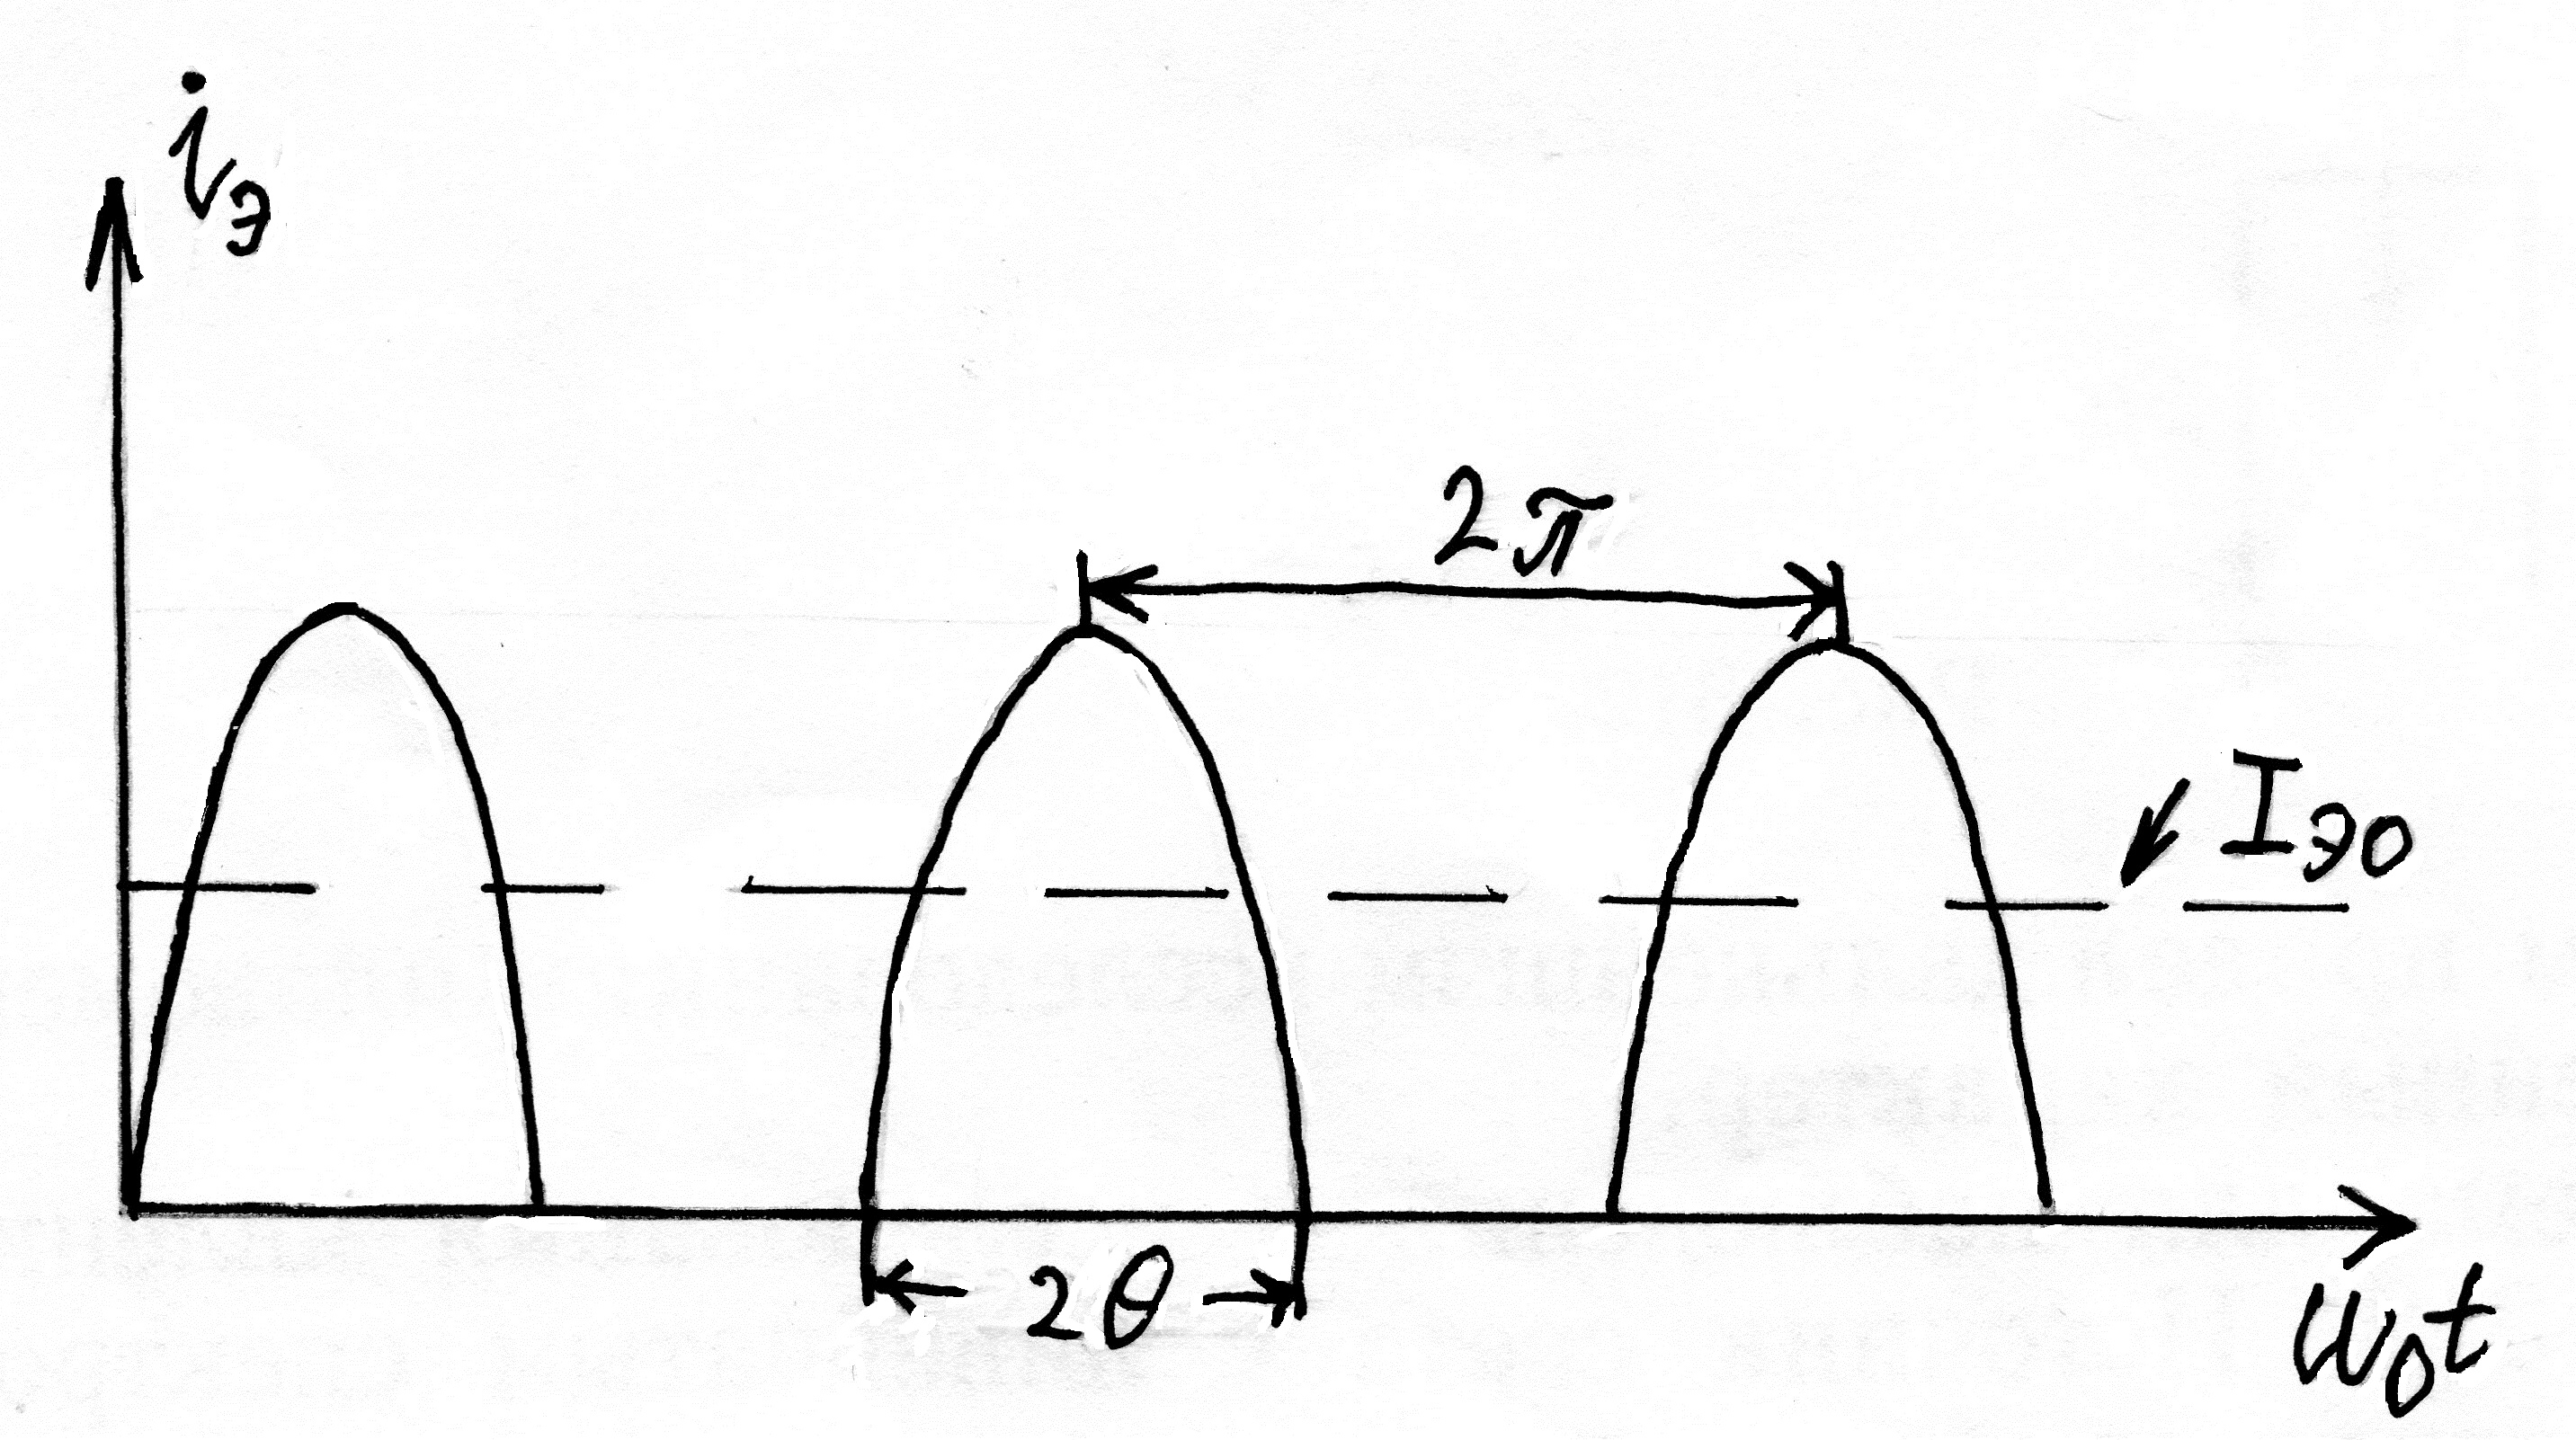
\includegraphics[width=\linewidth]{circuit/fig15}
\caption{}
\label{fig:fig15}
\vspace{-20pt}
\end{wrapfigure}

Результирующее постоянное напряжение между базой и эмиттером $U_\text{бэ}=E_\text{см}-U_\text{доп}$, где $E_\text{см}$ - начальное напряжение смещения между базой и эмиттером, задаемое с помощью делителя $R_1$ \textdiv $R_2$. Таким образом, рабочая точка транзистора будет смещаться в сторону меньших напряжений на базе, т.е. в область меньших углов отсечки. Это, во-первых, дает возможность работать транзистору в более выгодном энергетическом режиме, т.к. уменьшается постоянная составляющая тока коллектора и, следовательно, мощность источника питания, рассеиваемая на коллекторном переходе.

Во-вторых, уменьшается влияние транзистора на колебательный контур и тем самым повышается стабильность частоты автогенератора.
\section{Задание}
\begin{enumerate}
	\item Ознакомиться со схемой лабораторного макета генератора (см.Приложение) и измерительными приборами.
	\item Измерить частоту генерируемых колебаний, для чего
	\begin{enumerate}
		\item Переключатель "генератор-усилитель" поставить в положение "генератор";
		\item Включить емкость в цепи эмиттера;
		\item При минимальной связи установить на переходе база-эмиттер транзистора максимальное напряжение смещения $E_\text{см} = 0.7 B$. Отсчет $E_\text{см}$ производится по стрелочному индикатору на передней панели макета. Напряжение источника питания на коллекторе $E_k = 9 B$ и в процессе выполнения работы не изменяется;
		\item Увеличивая связь, добиться возбуждения генератора. Наличие автоколебаний регистрируется с помощью осциллографа и вольтметра, подключаемых соответственно к гнездам $\text{Г}_4$ и $\text{Г}_2$;
		\item Отключив осциллограф, подключить к гнезду $\text{Г}_4$ частотомер и измерить частоту автоколебаний при двух значениях емкости контура. Отключить дополнительную емкость от контура генератора.
	\end{enumerate}
	\item Снять зависимость амплитуды выходного напряжения от величины обратной связи для двух значений напряжения смещения $E_\text{см1}$ и $E_\text{см2}$; $E_\text{см1}$ соответствует положению начальной рабочей точки на участке с максимальной крутизной, а $E_\text{см2}$ - вблизи напряжения отсечки.
	\begin{enumerate}
		\item \underline{Напряжение смещения максимальное.}
		\begin{enumerate}
			\item К гнезду $\text{Г}_2$ подключить вольтметр, а к гнезду $\text{Г}_3$ - осциллограф.
			\item Установить максимальное напряжение $E_\text{см}$.
			\item Увеличивая и уменьшая коэффициент взаимоиндукции и между индуктивностью контура и индуктивностью связи, снять зависимости амплитуды напряжения на контуре $U_K=U_K(M)$ и постоянного напряжения между базой и эмиттером $U_\text{БЭ}=U_\text{БЭ}(M)$ от величины М.
			\item Зафиксировать характерные осциллограммы импульсов тока коллектора с указанием соответствующих им величин М.
			\item Повторить эти измерения при отключенной емкости в цепи эмиттера. 
		\end{enumerate}
		\item \underline{Напряжение смещения $E_\text{см} = 0$.}
		\begin{enumerate}
			\item Установить напряжение смещения $E_\text{см} = 0$.
			\item Установить максимальную обратную связь.
			\item Включить емкость в цепи эмиттера.
			\item Плавно увеличивая $E_\text{см}$, добиться возбуждения генератора. Изменяя связь, убедиться в наличии гистерезисной петли в зависимости $U_K=U_K(M)$.
			\item Уменьшая и увеличивая М, снять зависимости $U_K=U_K(M)$ и $U_\text{БЭ}=U_\text{БЭ}(M)$.
			\item Характерные осциллограммы импульсов тока зарисовать с указанием М, при которых они получены. 
		\end{enumerate}	
	\end{enumerate}	
	\item Снять колебательные характеристики при напряжениях смещения $E_\text{см1}$ и $E_\text{см2}$.
	\begin{enumerate}
		\item \underline{Напряжение смещения $E_\text{см} = 0$.}
		\begin{enumerate}
			\item Включить емкость в цепи эмиттера.
			\item Переключатель "генератор-усилитель" поставить в положение "усилитель".
			\item К гнезду $\text{Г}_1$ подключить внешний генератор синусоидальных колебаний.
			\item Частоту внешнего генератора подобрать такой, чтобы контур был настроен на резонанс. Для этого установить $U_\text{ВХ}\approx 0.05 B$. Изменяя частоту внешнего генератора добиться максимального отклонения стрелки вольтметра и максимальной амплитуды изображения на экране осциллографа, подключенного к гнезду $\text{Г}_4$.
			\item Изменяя $U_\text{ВХ}$ от 0.01 до 0.3 В, снять зависимости $U_K=U_K(M)$ и $U_\text{БЭ}=U_\text{БЭ}(U_\text{ВХ})$. С помощью подключенного к гнезду $\text{Г}_3$ осциллографа зафиксировать характерные осциллограммы тока коллектора и изменяя в его форме с указанием соответствующих им значении напряжения $U_\text{ВХ}$.
		\end{enumerate}
	Для исключения погрешностей рекомендуется проводить измерения при одном положении переключателя уровня выходного сигнала внешнего генератора - 0.3 В.
		\item \underline{Напряжение смещения $E_\text{см2}$.}
		\begin{enumerate}
				\item Не изменяя частоты внешнего генератора, установить $E_\text{см}=E_\text{см2}$. Для этого 
			    - переключатель "генератор-усилитель" поставить в положение "генератор";

			    - выполнить пункты i-iv раздела b задания 3 при включенной емкости $C_{\text{э}}$;

			    - установить переключатель "генератор-усилитель" вновь в положение "усилитель"; 
				\item Изменяя $U_\text{ВХ}$ от 0.01 до 0.3 В, снять зависимости $U_K=U_K(U_\text{ВХ})$ и $U_\text{БЭ}=U_\text{БЭ}(U_\text{ВХ})$. Зафиксировать характерные осциллограммы тока коллектора.
		\end{enumerate}
	\end{enumerate}
	\item Снять зависимость напряжения на контуре от частоты подаваемого на усилитель напряжения
		\begin{enumerate}  
			\item $E_{\text{см}} = E_{\text{см2}}$.
			\item Переключатель "генератор-усилитель" поставить в положение "усилитель".
			\item Изменяя частоту входного напряжения f в пределах от 20 кГц до значения f, несколько превышающего частоту генерации, измерить зависимость $U_K=U_K(f)$.
			\item Форму колебаний на выходе наблюдать с помощью осциллографа, подключенного к гнезду $\text{Г}_4$. 
		\end{enumerate}
\end{enumerate}
\section{Контрольные вопросы}
\begin{enumerate}
	\item Дать определение следующим понятиям:

	- комплексный коэффициент передачи линейного четырёхполюсника; 

	- амплитудно-частотная и фазо-частотная характеристики четырехполюсника;

	- крутизна вольт-амперной характеристики транзистора;

	- средняя крутизна резонансного усилительного каскада;

	- колебательная характеристика такого каскада.
	\item Как зависит средняя крутизна от смещения и от амплитуды входного синусоидального колебания?
	\item Как изменяется вид колебательной характеристики при изменении смещения?
	\item Как измерить колебательную характеристику?
	\item В чем заключаются условия самовозбуждения автогенератора?
	\item Чем определяется амплитуда стационарны колебаний автогенератора?
	\item При каких условиях колебания автогенератора приобретают стационарный характер?
	\item Какова форма коллекторного тока в стационарном режиме автогенератора?
	\item В чем заключается условие стационарности автогенератора?
	\item Может ли быть стационарное состояние автогенератора неустойчивым?
	\item Объяснить суть различия между мягким и жестким возбуждением автогенератора.
\end{enumerate}
\section{Приложение}

\begin{wrapfigure}{l}{0.4\linewidth}
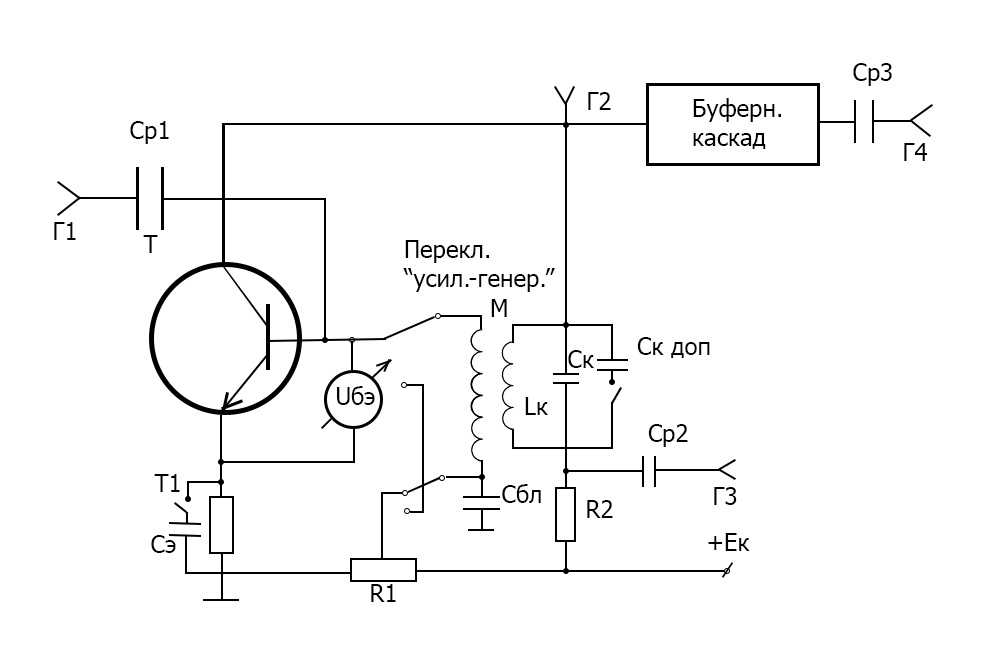
\includegraphics[width=\linewidth]{circuit/fig16}
\caption{}
\label{fig:fig15}
\vspace{-20pt}
\end{wrapfigure}

\section{Литература}
\begin{enumerate}
	\item Баскаков С.И. Радиотехнические цепи и сигналы.-М.: Высшая школа, 1983.
	\item Гоноровский И.С. Радиотехнические цепи и сигналы.-М.: Сов.радио, 1986.
	\item Основы теории колебаний. Под ред. Мигулина В.В.-М: Наука, 1976.
\end{enumerate}
\end{document}